\documentclass[12pt]{article}\usepackage[]{graphicx}\usepackage[dvipsnames]{xcolor}
\makeatletter
\def\maxwidth{ %
  \ifdim\Gin@nat@width>\linewidth
    \linewidth
  \else
    \Gin@nat@width
  \fi
}
\makeatother

\definecolor{fgcolor}{rgb}{0.345, 0.345, 0.345}
\newcommand{\hlnum}[1]{\textcolor[rgb]{0.686,0.059,0.569}{#1}}%
\newcommand{\hlstr}[1]{\textcolor[rgb]{0.192,0.494,0.8}{#1}}%
\newcommand{\hlcom}[1]{\textcolor[rgb]{0.678,0.584,0.686}{\textit{#1}}}%
\newcommand{\hlopt}[1]{\textcolor[rgb]{0,0,0}{#1}}%
\newcommand{\hlstd}[1]{\textcolor[rgb]{0.345,0.345,0.345}{#1}}%
\newcommand{\hlkwa}[1]{\textcolor[rgb]{0.161,0.373,0.58}{\textbf{#1}}}%
\newcommand{\hlkwb}[1]{\textcolor[rgb]{0.69,0.353,0.396}{#1}}%
\newcommand{\hlkwc}[1]{\textcolor[rgb]{0.333,0.667,0.333}{#1}}%
\newcommand{\hlkwd}[1]{\textcolor[rgb]{0.737,0.353,0.396}{\textbf{#1}}}%
\let\hlipl\hlkwb

\usepackage{framed}
\makeatletter
\newenvironment{kframe}{%
 \def\at@end@of@kframe{}%
 \ifinner\ifhmode%
  \def\at@end@of@kframe{\end{minipage}}%
  \begin{minipage}{\columnwidth}%
 \fi\fi%
 \def\FrameCommand##1{\hskip\@totalleftmargin \hskip-\fboxsep
 \colorbox{shadecolor}{##1}\hskip-\fboxsep
     \hskip-\linewidth \hskip-\@totalleftmargin \hskip\columnwidth}%
 \MakeFramed {\advance\hsize-\width
   \@totalleftmargin\z@ \linewidth\hsize
   \@setminipage}}%
 {\par\unskip\endMakeFramed%
 \at@end@of@kframe}
\makeatother

\definecolor{shadecolor}{rgb}{.97, .97, .97}
\definecolor{messagecolor}{rgb}{0, 0, 0}
\definecolor{warningcolor}{rgb}{1, 0, 1}
\definecolor{errorcolor}{rgb}{1, 0, 0}
\newenvironment{knitrout}{}{} % an empty environment to be redefined in TeX

\usepackage{alltt}
\usepackage{amsmath,amsfonts,amssymb,graphicx,authblk}
\usepackage[font={footnotesize,singlespacing},labelfont=bf]{caption}
\usepackage{titlesec,blkarray, bm} 
\usepackage{float,afterpage}
\usepackage[running,mathlines]{lineno}
\usepackage[vmargin=1in,hmargin=1in]{geometry}
\usepackage[authoryear,sort]{natbib}
\usepackage[dvipsnames]{xcolor}
\usepackage[nodisplayskipstretch]{setspace} 
\usepackage{hyperref}
\usepackage[section]{placeins}
\usepackage{gensymb}
\usepackage{enumitem}
\usepackage{orcidlink}
\setlist{topsep=.125em,itemsep=-0.15em,leftmargin=0.75cm}
\setlength{\parindent}{0.35in}

\usepackage[sc]{mathpazo} %Like Palatino with extensive math support
\usepackage[subtle]{savetrees}

\usepackage{lineno}

\clubpenalty = 10000
\widowpenalty = 10000

\sloppy 

\usepackage{ifpdf}
\ifpdf
\DeclareGraphicsExtensions{.pdf,.png,.jpg}
\usepackage{epstopdf}
\else
\DeclareGraphicsExtensions{.eps}
\fi

\graphicspath{{/Users/jm200/Library/CloudStorage/Dropbox/Miller Lab/github/POAR-Forecasting/Manuscript/Figures/}}
\newcommand{\tom}[2]{{\color{red}{#1}}\footnote{\textit{\color{red}{#2}}}}
\newcommand{\jacob}[2]{{\color{blue}{#1}}\footnote{\textit{\color{blue}{#2}}}}



% I cannot get \orcidlink working on my computer so for now replacing this with \textit

%-------------------------------------------------------------------------
\title{Forecasting range shifts of a dioecious plant species under climate change}
\author[1]{Jacob K. Moutouama\,\textit{0000-0003-1599-1671} \thanks{Corresponding author: jmoutouama@gmail.com}}
\author[2]{Aldo Compagnoni\,\textit{0000-0001-8302-7492}}
\author[1]{Tom E.X. Miller\,\textit{0000-0003-3208-6067}}
\affil[1]{Program in Ecology and Evolutionary Biology, Department of BioSciences, Rice University, Houston, Texas, USA}
\affil[2]{Institute of Biology, Martin Luther University Halle-Wittenberg, Halle, Germany; and German Centre for Integrative Biodiversity Research (iDiv), Leipzig, Germany}
\date{} % clear date
%\renewcommand\Authands{ and }

\sloppy

%-------------------------------------------------------------------------
\IfFileExists{upquote.sty}{\usepackage{upquote}}{}
\begin{document}
%\SweaveOpts{concordance=TRUE}
\renewcommand{\baselinestretch}{1.2}
\maketitle

\noindent\textbf{Running header:} Forecasting range shifts
\bigskip 

\noindent\textbf{Keywords:} demography, forecasting, global warming, matrix projection model, population dynamics, sex ratio, range limits

\bigskip 
\noindent\textbf{Submitted to:} \textit{Ecology letters} (Letter)

\bigskip 
\noindent\textbf{Data accessibility statement:} All data used in this paper are  publicly available and cited appropriately \citep{dryaddata}. 
Should the paper be accepted, all computer scripts supporting the results will be archived in a Zenodo package, with the DOI included at the end of the article. 
During peer review, our code (Stan and R) is available at \url{https://github.com/jmoutouama/POAR-Forecasting}. 

\bigskip 
\noindent\textbf{Conflict of interest statement:} None.

\bigskip
\noindent\textbf{Authorship statement:}
J.K.M., A.C. and T.E.X.M. designed the study.
A.C. and T.E.X.M. collected the data. 
All authors conducted the statistical analyses and modeling.
J.K.M. drafted the manuscript, and T.E.X.M contributed to revisions.

\bigskip
\noindent\textbf{Abstract:}\\
\noindent\textbf{Main Text:}\\
\noindent\textbf{Figures: 6}\\
\noindent\textbf{Tables: 0}\\
\noindent\textbf{References: 106}

\newpage
\linenumbers
%-------------------------------------------------------------------------
\spacing{1.25}
\section*{Abstract}
%150 words limit for Ecology letter. The number now is 155
%Tom made changes here that increase word count
Global climate change has triggered an urgent need for predicting the reorganization of Earth's biodiversity.
Currently, the vast majority of models used to forecast population viability and range shifts in response to climate change ignore the complication of sex structure, and thus the potential for females and males to differ in their sensitity to climate drivers. 
% For dioecious species, it is unclear how commonly unique climate sensitivities of females and males could influence projections for species-level responses to climate change. 
We developed demographic models of range limitation, parameterized from geographically distributed common garden experiments, with females and males of a dioecious grass species (\textit{Poa arachnifera}) throughout and beyond its range in the south-central U.S. 
Female-dominant and two-sex model versions both predict that future climate change will alter population viability and will induce a poleward niche shift beyond current northern limits.
However, the magnitude of niche shift was underestimated by the female-dominant model, because females have broader temperature tolerance than males and become mate-limited under female-biased sex ratios.
Our result illustrate how explicit accounting for both sexes could enhance population viability forecasts and conservation planning for dioecious species in response to climate change.

%--------------------------------------------------------------------
\newpage
\section*{Introduction}
Rising temperatures and extreme drought events associated with global climate change are leading to increased concern about how species will become redistributed across the globe under future climate conditions \citep{bertrand2011changes,gamelon2017interactions,smith2024extreme}.
Species' range limits, when not driven by dispersal limitation, should generally reflect the limits of the ecological niche \citep{lee2016synthesis}.
Niches and geographic ranges are often limited by climatic factors including temperature and precipitation \citep{sexton2009evolution}. 
Therefore, any substantial changes in the magnitude of these climatic factors could impact population viability, with implications for range expansions or contractions based on which regions of a species' range become more or less suitable  \citep{davis2001range, pease1989model}. 

%Dioecious species (most animals and ca. 7\% of plant species) might be particularly vulnerable to the influence of climate change because they often display skewed sex ratios that are generated or reinforced by sexual niche differentiation, i.e., the distinct responses of females and males to shared climate drivers) \citep{Tognetti2012}. 
Forecasting range shifts for dioecious species (most animals and ca. 7\% of plant species) is complicated by the potential for sexual niche differentiation, i.e. distinct responses of females and males to shared climate drivers \citep{Tognetti2012,pottier2021sexual,hultine2016climate,morrison2016causes}. 
The lower cost of reproduction for one sex (male or female) may allow that sex to invest its energy in other functions that produce higher growth rates, greater clonality, or even higher survival rates compared to the other sex, leading to sexual niche differentiation \citep{bruijning2017surviving}.
Accounting for sexual niche differentiation is a long-standing challenge in accurately predicting which sex will successfully track environmental change and how this will impact population viability and range shifts \citep{jones1999sex,gissi2023exploring}. 
Populations in which males are rare under current climatic conditions could experience low reproductive success due to sperm or pollen limitation that may lead to population decline in response to climate change that disproportionately favors females \citep{eberhart2017sex}.
In contrast, climate change could expand male habitat suitability (e.g. upslope movement), which might increase seed set for mate-limited females and favor range expansion \citep{petry2016sex}. 
Across dioecious plants, for example, studies suggest that future climate change toward hotter and drier conditions may favor male-biased sex ratios \citep{field2013comparative,hultine2016climate}. 
Although the response of species to climate warming is an urgent and active area of research, few studies have disentangled the interaction between sex and climate drivers to understand their combined effects on population dynamics and range shifts, despite calls for such an approach \citep{hultine2016climate,gissi2023exploring}.

The vast majority of theory and models in population biology, including those used to forecast biodiversity responses to climate change, ignore the complication of sex structure \citep[but see][] {pottier2021sexual,ellis2017does,Elena}.
Traditional approaches instead focus exclusively on females, assuming that males are in sufficient supply as to never limit female fertility. 
In contrast, ``two-sex'' models are required to fully account for demographic differences between females and males and sex-specific responses to shared climate drivers \citep{gerber2014two,miller2011sex}. 
Sex differences in maturation, reproduction, and mortality schedules can generate skew in the operational sex ratio (OSR; sex ratio of individuals available for mating) even if the birth sex ratio is 1:1 \citep{eberhart2017sex,shelton2010ecological}. 
Climate and other environmental drivers can therefore influence the OSR via their influence on sex-specific demographic rates. 
In a two-sex framework, demographic rates both influence and respond to the OSR in a feedback loop that makes two-sex models inherently nonlinear and more data-hungry than corresponding female-dominant models. 
Given the additional complexity and data needs, forecasts of range dynamics for dioecious species under future climate change that explicitly account for females, males, and their inter-dependence are limited \citep{petry2016sex,lynch2014climate}.


% \tom{Climate change can influence dioecious populations via shifts in sex ratio.}{This paragraph is really good but notice that the topic sentence (and much that follows) is largely redundant with the first paragraph. I would suggest creating clearer distinction between paragraphs.} 
% Females and males may respond differently to climate change, especially in species where there is sexual niche differentiation \citep{gissi2023exploring,gissi2023sex,hultine2016climate}. 
% This sex-specific response to climate change may help one sex to succeed in extreme climatic conditions rather than the other sex \citep{zhao2012sex, burli2022environmental} leading to a skewness in the operational sex ratio (relative number of males and females as available mates) \citep{eberhart2017sex}.
% For example, experiments in two populations of Atlantic marine copepods (\textit{Acartia tonsa}) revealed that male survival was more sensitive to increasing temperatures than female survival \citep{sasaki2019complex}.
% In other species, such as \textit{Pteropus poliocephalus} or \textit {Populus cathayana}, females showed lower survival than males in response to high temperature \citep{welbergen2008climate,zhao2012sex}. 
% Sex-specific responses to climate drivers have the potential to influence population viability under global change because skew in the operational sex ratio can limit reproduction through mate scarcity \citep{petry2016sex}.

Tracking the impact of climate change on  population viability ($\lambda$) and distributional limits of dioecious taxa depends on our ability to build mechanistic models that take into account the spatial and temporal context of sex specific response to climate change, while accounting for sources of uncertainty \citep{davis2001range,evans2016towards}.
Structured population models built from demographic data collected from geographically distributed observations or common garden experiments provide several advantages for studying the impact of climate change on species' range shifts \citep{merow2017climate,schwinning2022common,schultz2022climate}.
First, demographic models link individual-level life history events (mortality, development, and regeneration) to population demography, allowing the investigation of factors explaining vital rate responses to environmental drivers \citep{ehrlen2015predicting,louthan2022climate,dahlgren2016demography}. 
Second, demographic models have a natural interface with %experimental treatments that can isolate spatial and temporal correlations between environmental factors, thus overcoming a main disadvantage with many types of correlative studies \citep{leicht2007comparative}. 
%Third, demographic models are typically constructed from 
statistical estimation of individual-level vital rates that provide quantitative measures of uncertainty and isolate different sources of variation, features that can be propagated to population-level predictions \citep{elderd2016quantifying,ellner2022critical}.
% The uncertainty around lambda can be used to estimate the probability of self-sustaining populations, conditional on different factors of the environment.
Finally, structured demographic models can be used to identify which aspects of climate are the most important drivers of population dynamics.
For example, Life Table Response Experiments (LTRE) built from structured models have become widely used to understand the relative importance of covariates in explaining variation in population growth rate  \citep{ellner2016data,hernandez2023exact,czachura2020demographic}.
%LTRE is also used to get a mechanistic understanding of how a given treatment (eg. temperature or precipitation) could affect population dynamics through unique vital rate responses \citep {caswell1989analysis,o2024nonlinear,morrison2007demographic,iler2019reproductive}. %\jacob{}{Yes I don't want to get distracted by SDMs. The story is still interesting without bashing the SDMs studies. That being said, I showed the advantage of using demographic models over traditional correlative approaches. Line 59-62)}
% At their range edge where climatic conditions are expected to be less favorable, if dioecious species populations are non-viable in response to climate change, global warming will induce range contraction in dioecious species.
% In reverse, if populations at the edge are viable habitats in response to global warming, dioecious species populations could shift their range and relocate to more favorable and thereby favored range expansion. 

In this study, we combined geographically-distributed common garden experiments, hierarchical Bayesian statistical modeling, two-sex population projection modeling, and climate back-casting and forecasting to understand demographic responses to climate change and their implications for past, present, and future range dynamics. 
Our work focused on the dioecious plant Texas bluegrass (\textit{Poa arachnifera}), which is distributed along environmental gradients in the south-central U.S. corresponding to variation in temperature across latitude and precipitation across longitude (Fig. \ref{fig:study_design}A)\jacob{}{Fig. A  does not show what we are saying here. Maybe I should add the Figure with the raster}. 
This region has experienced rapid climate warming since 1900 and this is projected to continue through the end of the century (Fig. \ref{fig:study_design} B and C). 
Our previous study showed that, despite evidence for differentiation of climatic niche between sexes, the female niche mattered the most in driving longitudinal range limits of Texas bluegrass \citep{miller2022two}. 
However, that study used a single proxy variable (longitude) to represent environmental variation related to aridity and did not consider variation in temperature, which is the much stronger dimension of forecasted climate change in this region (Fig. \ref{Sup:climate_normal_weather}). 
Developing a rigorous forecast for the implications of future climate change requires that we transition from implicit to explicit treatment of multiple climate drivers, as we do here.
Leveraging the power of Bayesian inference, we take a probabilistic view of past, present, and future range limits by quantifying the probability of population viability ($Pr(\lambda\ge1)$) in relation to climate drivers of demography, an approach that fully accounts for uncertainty arising from multiple sources of estimation and process error. %using Markov Chain Monte Carlo (MCMC) can be utilized to infer species niche which is defined as the range of resources and conditions allowing its populations of self-sustaining populations, conditional on different factors of the environment \citep{maguire1973niche,hutchinson1978introduction,diez2014probabilistic}
Specifically, we asked: 
\begin{enumerate}
	\item What are the sex-specific vital rate responses to variation in temperature and precipitation across the species' range?
	\item How do sex-specific vital rates combine to determine the influence of climate variation on population growth rate ($\lambda$)?
	\item What is the impact of climate change on operational sex ratio throughout the range?
	\item What are the likely historical and projected dynamics of the Texas bluegrass geographic niche and how does accounting for sex structure modify these predictions?
\end{enumerate}

%--------------------------------------------------------------------
\section*{Materials and methods}
\subsection*{Study species and climate context}
Texas bluegrass (\textit{Poa arachnifera}) is a dioecious perennial, summer-dormant cool-season (C3) grass that occurs in the south-central U.S. (Texas, Oklahoma, and southern Kansas) (Figure \ref{fig:study_design}) \citep{hitchcock1971manual}. 
Texas bluegrass grows between October and May, flowers in spring, and goes dormant during the hot summer months of June to September \citep{kindiger2004interspecific}. 
Following this life history, we divided the calendar year into growing (October 1 - May 31) and dormant (June 1 - September 30) seasons in the analyses below. 
Biological sex is genetically based and the birth (seed) sex ratio is 1:1 \citep{renganayaki2005identification}. 
Females and males are morphologically indistinguishable except for their inflorescences. 
Like all grasses, this species is wind pollinated \citep{hitchcock1971manual} and most male-female pollen transfer occurs within 10-15m \citep{compagnoni2017can}. 
Surveys of 22 natural populations throughout the species' distribution indicated that operational sex ratio (the female fraction of inflorescences) ranged from 0.007 to 0.986 with a mean of 0.404 \citep{miller2022two}. 

Latitudinal limits of the Texas bluegrass distribution span 7.74 \degree C to 16.94 \degree C of temperature during the dormant season and 24.38 \degree C to 28.80 \degree C  during the dormant season. 
Longitudinal limits span 244.9 mm to 901.5 mm of precipitation during the growing season and 156.3 mm to 373.3 mm. 
This region has experienced \textit{ca.} 0.5 \degree C of climate warming since 1900, with faster warming  during the cool-season months ($0.0055 \degree C / yr$) than the hot summers ($0.0046\degree C / yr$) (Fig. \ref{Sup:climate_variation1}).
Future warming is projected to accelerate to $0.03-0.06\degree C / yr$ by the end of the century depending on the season and forecast model. 
On the other hand, precipitation has increased over the past century for much of the region but is forecasted to decline back to early-20th century levels (Fig. \ref{Sup:climate_variation1}). 
\jacob{}{I like this but I don't know if this not a repetition of what we've said in the introduction about climate change in the study area. }

\subsection*{Common garden experiment}
\subsubsection*{Experimental design}
We conducted a range-wide common garden experiment to quantify sex-specific demographic responses to climate variation. 
Details of the experimental design are provided in \cite{miller2022two}; we provide a brief overview here. 
The experiment was installed at 14 sites throughout and, in some cases, beyond the natural range of Texas bluegrass that sampled a broad range of latitude and longitude (Figure \ref{fig:study_design}A).
At each site, we established 14 blocks. 
For each block we planted three female and three male individuals that were clonally propagated from females and males from eight natural source populations (Figure \ref{fig:study_design}A); because sex is genetically-based, clones never deviated from their expected sex. 
The experiment was established in November 2013 with a total of 588 female and 588 male plants, and was censused in May of 2014, 2015, and 2016. 
At each census, we collected data on survival, size (number of tillers), and number of panicles (reproductive inflorescences). 
For the analyses that follow, we focus on the 2014-15 and 2015-16 transition years, since the start of the experiment did not include the full 2013-14 transition year. 

\begin{figure}[H]
  \begin{center}
    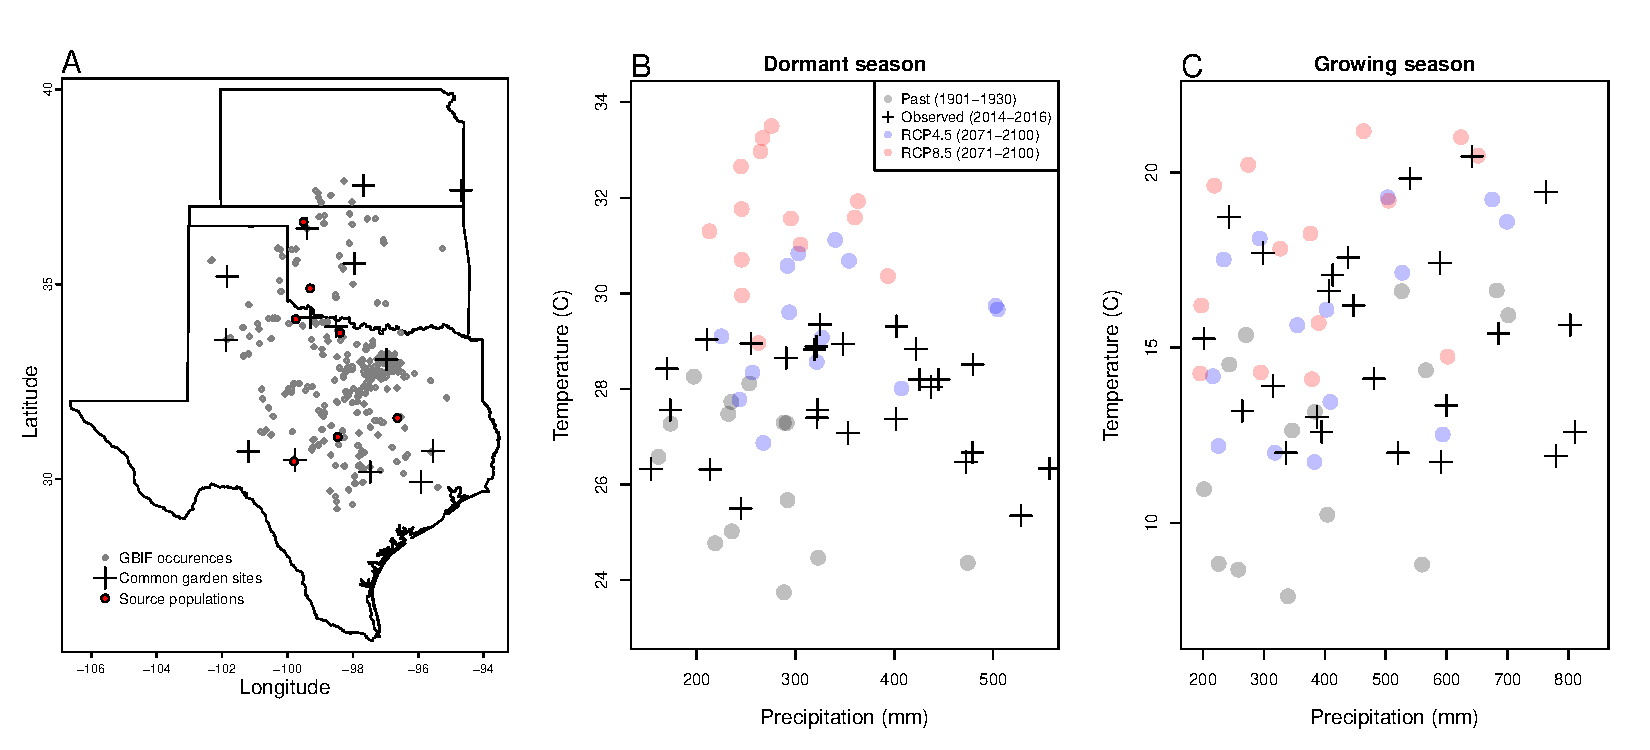
\includegraphics[width=1\linewidth]{Figures/tom_map_v2.pdf}
  \caption{\textbf{Experimental gardens and climate of the study region}. 
  	\textbf{A}: Map of 14 experimental garden sites (crosses) in Texas, Oklahoma, and Kansas relative to GBIF occurrences of \textit{Poa arachnifera} (gray points). Red points indicate source populations for plants used in the common garden experiment. 
  	\textbf{B,C}: Past, future, and observed climate space for growing and dormant seasons. Crosses show observed conditions for the sites and years of the common garden experiment. Gray points show historical (1901-1930) climate normals, and blue and red points show end-of-century (2071-2100) climate normals for RCP4.5 and RCP8.5 projections, respectively, form MIROC5. 
  See also (Figure \ref{Sup:clim_change} for more information about historical and projected climate change in the study region.}
  \label{fig:study_design}
  \end{center}
\end{figure}

\subsubsection*{Climatic data collection}
We gathered downscaled monthly temperature and precipitation for each site from Chelsa \citep{karger2017climatologies} to describe observed climate conditions during our study period.
These climate data were used as covariates in vital rate regressions. 
%We prefer temperature and precipitation because they capture the most the climate in the study region \colorbox{BurntOrange}{Source}. 
We aligned the climatic years to match demographic transition years (June 1 -- May 31) and growing and dormant seasons within each year.
%Based on the natural history of this summer-dormant cool-season species, we divided each transition year into dormant (June 1 through September 30) and growing (October 1 through May 31) seasons. 
% The 2014-15 transition year was substantially wetter and cooler across the study region than 2015-16, especially during the growing season (Fig.\ref{Sup:climate_variation}), so our study design provides both spatial and inter-annual coverage of climate variables. 
To back-cast and forecast demographic responses to changes in climate throughout the study region, we also gathered projection data for three 30-year periods: ``past'' (1901-1930), ``current'' (1990-2019) and ``future'' (2070-2100).
Data for future climatic periods were downloaded from four general circulation models (GCMs) selected from the Coupled Model Intercomparison Project Phase 5 (CMIP5): Model for Interdisciplinary Research on Climate (MIROC5), Australian Community Climate and Earth System Simulator (ACCESS1-3), Community Earth System Model (CESM1-BGC), Centro Euro-Mediterraneo sui Cambiamenti Climatici Climate Model (CMCC-CM).
All the GCMs were also downloaded from Chelsa \citep{sanderson2015representative}.
We evaluated future climate projections from two scenarios of representative concentration pathways (RCPs): RCP4.5, an intermediate-to-pessimistic scenario assuming a radiative forcing amounting to 4.5 $W m^{-2}$ by 2100, and RCP8.5, a pessimistic emission scenario which projects a radiative forcing of 8.5 $W m^{-2}$ by 2100 \citep{thomson2011rcp4, schwalm2020rcp8}. 

Projection data for the three 30-year periods included warmer or colder conditions than observed in our experiment, so extending our inferences to these conditions required some extrapolation. 
However, across all sites, both study years were 1-2\degree C warmer than their corresponding ``current'' (1990-2019) temperature normals (Fig. \ref{Sup:climate_normal_weather}). 
Additionally, the 2014--15 growing season was generally wetter and cooler across the study region than 2015--16 (Fig. \ref{Sup:climate_normal_weather}). 
Combined, the geographic and inter-annual replication of the common garden experiment provided good coverage of most past and future conditions throughout the study region (Fig. \ref{fig:study_design}B,C). 

\subsubsection*{Sex-specific demographic responses to climatic variation across common garden sites}
We used individual-level measurements of survival, growth (change in number of tillers), flowering, and number of panicles (conditional on flowering) to develop Bayesian mixed effect models describing how each vital rate varies as a function of sex, size, and four climate covariates (precipitation and temperature of growing and dormant season)(Supplementary Method \ref{sssec:vital_rate}). 
%\tom{We kept the four climate covariates in the mixed effect models because each climatic variable describes different aspect of climate that could be important for the species persistence across its range.}{This sentence does not contain any information.} 
These vital rate models included main effects of size (the natural log of tiller number), sex, and seasonal climate covariates. 
Climate variables were fit with second-degree polynomial functions to accommodate the possibility of hump-shaped relationships (reduced demographic performance at both extremes).
We also included two-way interactions between sex and each climate driver and between temperature and precipitation within each season, and a three-way interaction between sex, temperature, and precipitation within each season. 
We modeled survival and flowering data with a Bernoulli distribution and the growth (tiller number) with a zero-truncated Poisson inverse Gaussian distribution. 
Fertility (panicle count conditional on flowering) was modeled as zero-truncated negative binomial. 
We used generic, weakly informative priors to fit coefficients for survival, growth, flowering models ($\beta \sim N(0,\ 1.5)$) and random effect variances ($\sigma \sim Gamma(\gamma (0.1,\ 0.1)$).
We fit fertility model with  also weakly informative priors for coefficients ($\beta \sim N(0,\ 0.15)$).
Different priors  were used for fertility because the panicle model has a large number of parameters relative to the amount of available data (subset of our data) and because these specifics priors help  prevent the model from overfitting. 
Each vital rate also includes normally distributed random effects for block-to-block variation ($\phi \sim N(0,\ \sigma_{block})$), site to site variation ($\nu \sim N(0,\ \sigma_{site})$), and source-to-source variation that is related to the genetic provenence of the transplants used to establish the common garden ($\rho \sim N(0,\ \sigma_{source})$).


\subsubsection*{Sex ratio responses to climatic variation across common garden sites}
We also used the experimental data to investigate how climatic variation across the range influenced sex ratio and operational sex ratio of the common garden populations. 
To do so, we developed  two Bayesian linear models using  data collected during three years.
Each model had OSR or SR as response variable and a climate variable (temperature and precipitation of the growing season and dormant season) as predictor (Supplementary Method \ref{sssec:sexratio_bayesian}). 
We modeled the OSR or SR data with a Bernoulli distribution and used non informative priors for each coefficient ($\omega \sim N(0,\ 100)$). 

\subsubsection*{Model-fitting procedures}
All models were fit using Stan \citep{rstan} in R 4.3.1 \citep{RCoreteam}.
We centered and standardized all climatic predictors to mean zero, variance one, which facilitated model convergence.
We ran three chains for 1000 samples for warmup and 4000 for sampling, with a thinning rate of 3.
We assessed the quality of the models using posterior predictive checks \citep{piironen2017comparison} (Figure \ref{Sup:PPC}).
%To understand the effect of climate on vital rates, we got the 95 \% credible interval of the posterior distribution. 
%Then we assumed that there is 95 \% probability that the true (unknown) estimates would lie within that interval, given the evidence provided by the observed data for each vital rate.
 
\subsection*{Two-sex and female-dominant matrix projection models}
We used the climate-dependent vital rate regressions estimated above, combined with additional data sources, to build female-dominant and two-sex versions of a climate-explicit matrix projection model (MPMs) structured by the discrete state variables size (number of tillers) and sex.
The female-dominant and two-sex versions of the model both allow for sex-specific response to climate and differ only in the feedback between operational sex ratio and seed fertilization. 
For clarity of presentation we do not explicitly include climate-dependence in the notation below, but the following model was evaluated over variation in seasonal temperature and precipitation. 

Let $F_{x,\ t}$ and $M_{x,\ t}$ be the number of female and male plants of size $x$ in year $t$, where $x \in [1,...\ U]$.
The minimum possible size is one tiller and $U$ is the 95th percentile of observed maximum size (35 tillers).
Let $F^{R}_{t}$ and $M^{R}_{t}$ be new female and male recruits in year $t$, which we treat as distinct from the rest of the size distribution because we assume they do not reproduce in their first year, consistent with our observations.
For a pre-breeding census, the expected numbers of recruits in year $t+1$ is given by:
\begin{align}\label{eq:recruits}
F^{R}_{t+1} = \sum_{1}^{U} 	[ \, p^{F}(x) \cdot c^{F}(x) \cdot d \cdot v(\mathbf{F_{t}},\ \mathbf{M_{t}}) \cdot m \cdot \rho 	] \, F_{x,\ t}
\\
M^{R}_{t+1} = \sum_{1}^{U} 	[ \, p^{F}(x) \cdot c^{F}(x) \cdot d \cdot v(\mathbf{F_{t}},\ \mathbf{M_{t}}) \cdot m \cdot (1-\rho) 	] \, F_{x,\ t}
\end{align}
\noindent where $p^{F}$ and $c^{F}$ are flowering probability and panicle production for females of size $x$, $d$ is the number of seeds per female panicle, $v$ is the probability that a seed is fertilized, $m$ is the probability that a fertilized seed germinates, and $\rho$ is the primary sex ratio (proportion of recruits that are female), which we assume to be $0.5$ \citep{miller2022two}. 

In the two-sex model, seed fertilization is a function of population structure, allowing for feedback between vital rates and operational sex ratio (OSR). 
In the context of the model, OSR is defined as the fraction of panicles that are female and is derived from the $U \times 1$ vectors $\mathbf{F_{t}}$ and $\mathbf{M_{t}}$:
\begin{align}\label{eq:viab_MPM}
	v(\mathbf{F_{t}},\mathbf{M_{t}}) = v_{0} * \left[ 1 - \left( \frac{\sum_{1}^{U} p^{F}(x,\ z) c^{F}(x,\ z) F_{x,t}}{\sum_{1}^{U} p^{F}(x,\ z) c^{F}(x,\ z) F_{x,t} + p^{M}(x,\ z) c^{M}(x,\ z) M_{x,\ t}} \right) ^{\alpha}\right]
\end{align}
The summations tally the total number of female and male panicles over the size distribution, giving the fraction of total panicles that are female. 
We focus on the female fraction of panicles and not female fraction of reproductive individuals because panicle number can vary widely depending on size; we assume that few males with many panicles vs. many males with few panicles are interchangeable pollination environments. 
Eq. \ref{eq:viab_MPM} has the properties that seed fertilization is maximized at $v_{0}$ as OSR approaches 100\% male, goes to zero as OSR approaches 100\% female, and parameter $\alpha$ controls how female seed viability declines as male panicles become rare. 
We estimated these parameters using data from a sex ratio manipulation experiment, conducted in the center of the range, in which seed fertilization was measured in plots of varying OSR; this experiment is described elsewhere  \citep{compagnoni2017can} and is summarized in \tom{Supplementary Method \ref{sssec:experiment}}{I think the supplement should also include a data figure showing the fit of the model to the experimental data.}. 
This experiment also provided estimates for seed number per panicle ($d$) and germination rate ($m$). 
Lacking data on climate-dependence, we assume that seed fertilization, seed number, and germination rate do not vary with climate.  

The dynamics of the size-structured component of the population are given by:
\begin{align}\label{eq:dynamics}
F_{y,t+1} = [ \, \sigma \cdot g^{F}(y,\ x=1) ] \, F^{R}_{t} + \sum_{L}^{U} 	[ \, s^{F}(x) \cdot g^{F}(y,\ x)] \, F_{x,\ t}
\\
M_{y,t+1} = [ \, \sigma \cdot g^{M}(y,\ x=1) ] \, M^{R}_{t} + \sum_{L}^{U} 	[ \,  s^{M}(x) \cdot g^{M}(y,\ x) ] \, M_{x,\ t}
\end{align}

\noindent The first terms indicate recruits that survived their first year and enter the size distribution of established plants.
We estimated the seedling survival probability $\sigma$ using demographic data from the congeneric species \textit{Poa autumnalis} in east Texas (T.E.X. Miller and J.A. Rudgers, \textit{unpublished data}), and we assume that $\sigma$ is the same across sexes and climatic variables. 
We did this because we had little information on the early life cycle transitions of greenhouse-raised transplants.
We used $g\ (y,\ x=1)$ (the future size distribution of one-tiller plants from the transplant experiment) to give the probability that a surviving recruit reaches size $y$.
The second component of the equations indicates survival and size transition of established plants from the previous year, where $s$ and $g$ give the probabilities of surviving at size $x$ and growing from sizes $x$ to $y$, respectively, and superscripts indicate that these functions may be unique to females ($F$) and males ($M$).

The model described above yields a $2(U+1) \times 2(U+1)$ transtion matrix. 
We estimated the population growth rate $\lambda$ of the female dominant model as the leading eigenvalue of the transition matrix. 
Since the two-sex MPM is nonlinear (matrix elements affect and are affected by population structure) we estimated $\lambda$ and stable sex ratio (female fraction of all individuals) and operational sex ratio (female fraction of panicles) by numerical simulation.
Since all parameters were estimated using MCMC sampling, we were able to propagate the uncertainty in our estimates of the vital rate parameters to uncertainty in $\lambda$. 
Furthermore, by sampling over distributions associated with site, block, and source population variance terms, we are able to incorporate process error into the total uncertainty in $\lambda$, in addition to the uncertainty that arises from imperfect knowledge of the parameter values. 
For example, sampling over site and block variances accounts for regional and local spatial heterogeneity that is not explained by climate, and sampling over source population variance accounts for genetically-based demographic differences across the species' range.


\subsection*{Life Table Response Experiments}
%\jacob{}{I modified this section. I understand your concern about accounting for the second order term in the first LTRE but I don't think we should be worry about that here. I am saying that because the technic here is similar to an ANOVA-- we dropped one predictor to see how much the error goes up. That's why we don't account for sex or size because lambda account for them already.}
We conducted two types of Life Table Response Experiments (LTRE) to isolate contributions of climate variables and sex-specific vital rates to variation in $\lambda$.
First, to identify which aspect of climate is most important for population viability, we used an LTRE based on a nonparametric model for the dependence of $\lambda$ on parameters associated with seasonal temperature and precipitation \citep{ellner2016data}. 
To do so, we used the RandomForest package to fit a regression model with four climatic variables (temperature of growing season, precipitation of growing season, temperature of the dormant season and precipitation of the dormant season) as predictors  and $\lambda$  calculated from the two sex model as response \citep{liaw2002classification}.
The regression model allowed the estimation of the relative importance of each predictor. 
%\jacob{The importance of each climate covariate is measured by asking: how wrongly is $\lambda$ predicted if we replaced the focal predictor (e.g., temperature of growing season) by a random value of the other predictors.}{hope this makes sense now}

Second, to understand how climate drivers influence $\lambda$ via sex-specific demography, we decomposed the effect of each climate variable on population growth rate ($\lambda$) into contribution arising from the effect on each female and male vital rate using a ``regression design'' LTRE \citep{caswell1989analysis,caswell2000matrix}.
This LTRE decomposes the sensitivity of $\lambda$ to climate according to:

\begin{align}\label{eq:ltresex}
\frac{\partial \lambda}{\partial climate} \approx \sum_{i} \frac{\partial \lambda}{\partial \theta^{F}_{i}} \frac{\partial \theta^{F}_{i}}{\partial climate} + \frac{\partial \lambda}{\partial \theta^{M}_{i}} \frac{\partial \theta^{M}_{i}}{\partial climate}
\end{align}

\noindent where, $\theta^{F}_{i}$ and $\theta^{M}_{i}$ represent sex-specific parameters (the regression coefficients of the vital rate functions). 
Because LTRE contributions are additive, we summed across vital rates to compare the total contributions of female and male parameters.
\jacob{}{Let's talk about this}\tom{}{I do not agree. It is true that you can compute this, but only by ``turning off'' the interaction by holding the interacting variable constant. I still think this needs to be better addressed in both LTRE analyses.}

\subsection*{Population viability across the climatic niche and geographic range}
% A species' ecological niche can be defined as the range of resources and conditions allowing its populations to self- sustained  ($\lambda > 1$) \citep{maguire1973niche,hutchinson1978introduction,diez2014probabilistic}.
To understand how climate shapes the niche and geographic range of Texas bluegrass, we estimated the probability of self- sustaining populations (Pr ($\lambda \ge 1$)) conditional to temperature and precipitation of the dormant and growing seasons.
Pr ($\lambda > 1$) was calculated for the two-sex model and the female dominant MPMs using the proportion of the 300 posterior samples that lead to a $\lambda \ge 1$ \citep{diez2014probabilistic}.
Population viability in climate niche space was then represented as a contour plot with values of Pr ($\lambda > 1$) at given temperature and precipitation for the growing season, holding dormant season climate constant, and vice versa. 
%We also visualized how our common garden sites have moved and are expected to move through climate space through time due to climate change. 

Pr ($\lambda > 1$) was also mapped onto geographic layers of three US states (Texas, Oklahoma and Kansas) to delineate past, current and future potential geographic distribution of the species.
To do so, we estimated Pr ($\lambda > 1$) conditional to all climate covariates for each pixel ($\sim$25 km2) for each time period (past, present, future).
Because of the amount of the computation involved, we use 100 posterior samples to estimate Pr ($\lambda > 1$) across the study area (Texas, Oklahoma and Kansas).

%\tom{To compare the probability of self-sustaining populations between the female dominant and the two-sex model, we used a zero-inflated beta model in brms \citep{brms}. }{This just floats here without much context. Not sure we need it, but I am flagging for now and will come back to this after reading the results.}

\section*{Results}

\subsection*{Sex specific demographic response and sex ratio variation across climatic conditions}
We found strong demographic responses to climate drivers across our Texas bluegrass common garden sites and years, and evidence for demographic differences between the sexes. 
Regression coefficients related to sex and/or sex:size interactions were significantly non-zero (95\% credible intervals excluding zero) for most vital rates (Fig. \ref{Sup:Posterior}), suggesting sexual divergence in demography. 
Females generally had an advantage over males, especially in survival and flowering (Fig. \ref{fig:vital_rates}). 
\jacob{That female demographic advantage was more pronounce for extreme values of climate (Fig. \ref{Sup:vt_3D_grow}, Fig. \ref{Sup:vt_3D_dorm}).}{I added the 3D plots for vital rates to show that female individuals do better in extreme  climate}
Vital rate regressions also revealed significant interactions between sex and climate drivers, especially in vegetative growth (Fig. \ref{Sup:Posterior})B. 
\tom{}{I am skipping the rest of this section for now because I think we need a different visualization for the vital rates. I also think this section should include the common garden sex ratio results, since they are connected to the vital rate responses.}


% Plant size and sex interaction was significant for all vitals rates (Fig. \ref{Sup:Posterior}), suggesting a sexual dimorphism.
% For survival, flowering and reproduction the interaction between temperature and precipitation of the growing season and dormant season was not significant (Fig. \ref{Sup:Posterior}). 
% However, for growth, the interaction between temperature and precipitation of the growing season and dormant season was significantly higher than zero (Fig. \ref{Sup:Posterior}). 

\begin{figure}[H]
	\begin{center}
		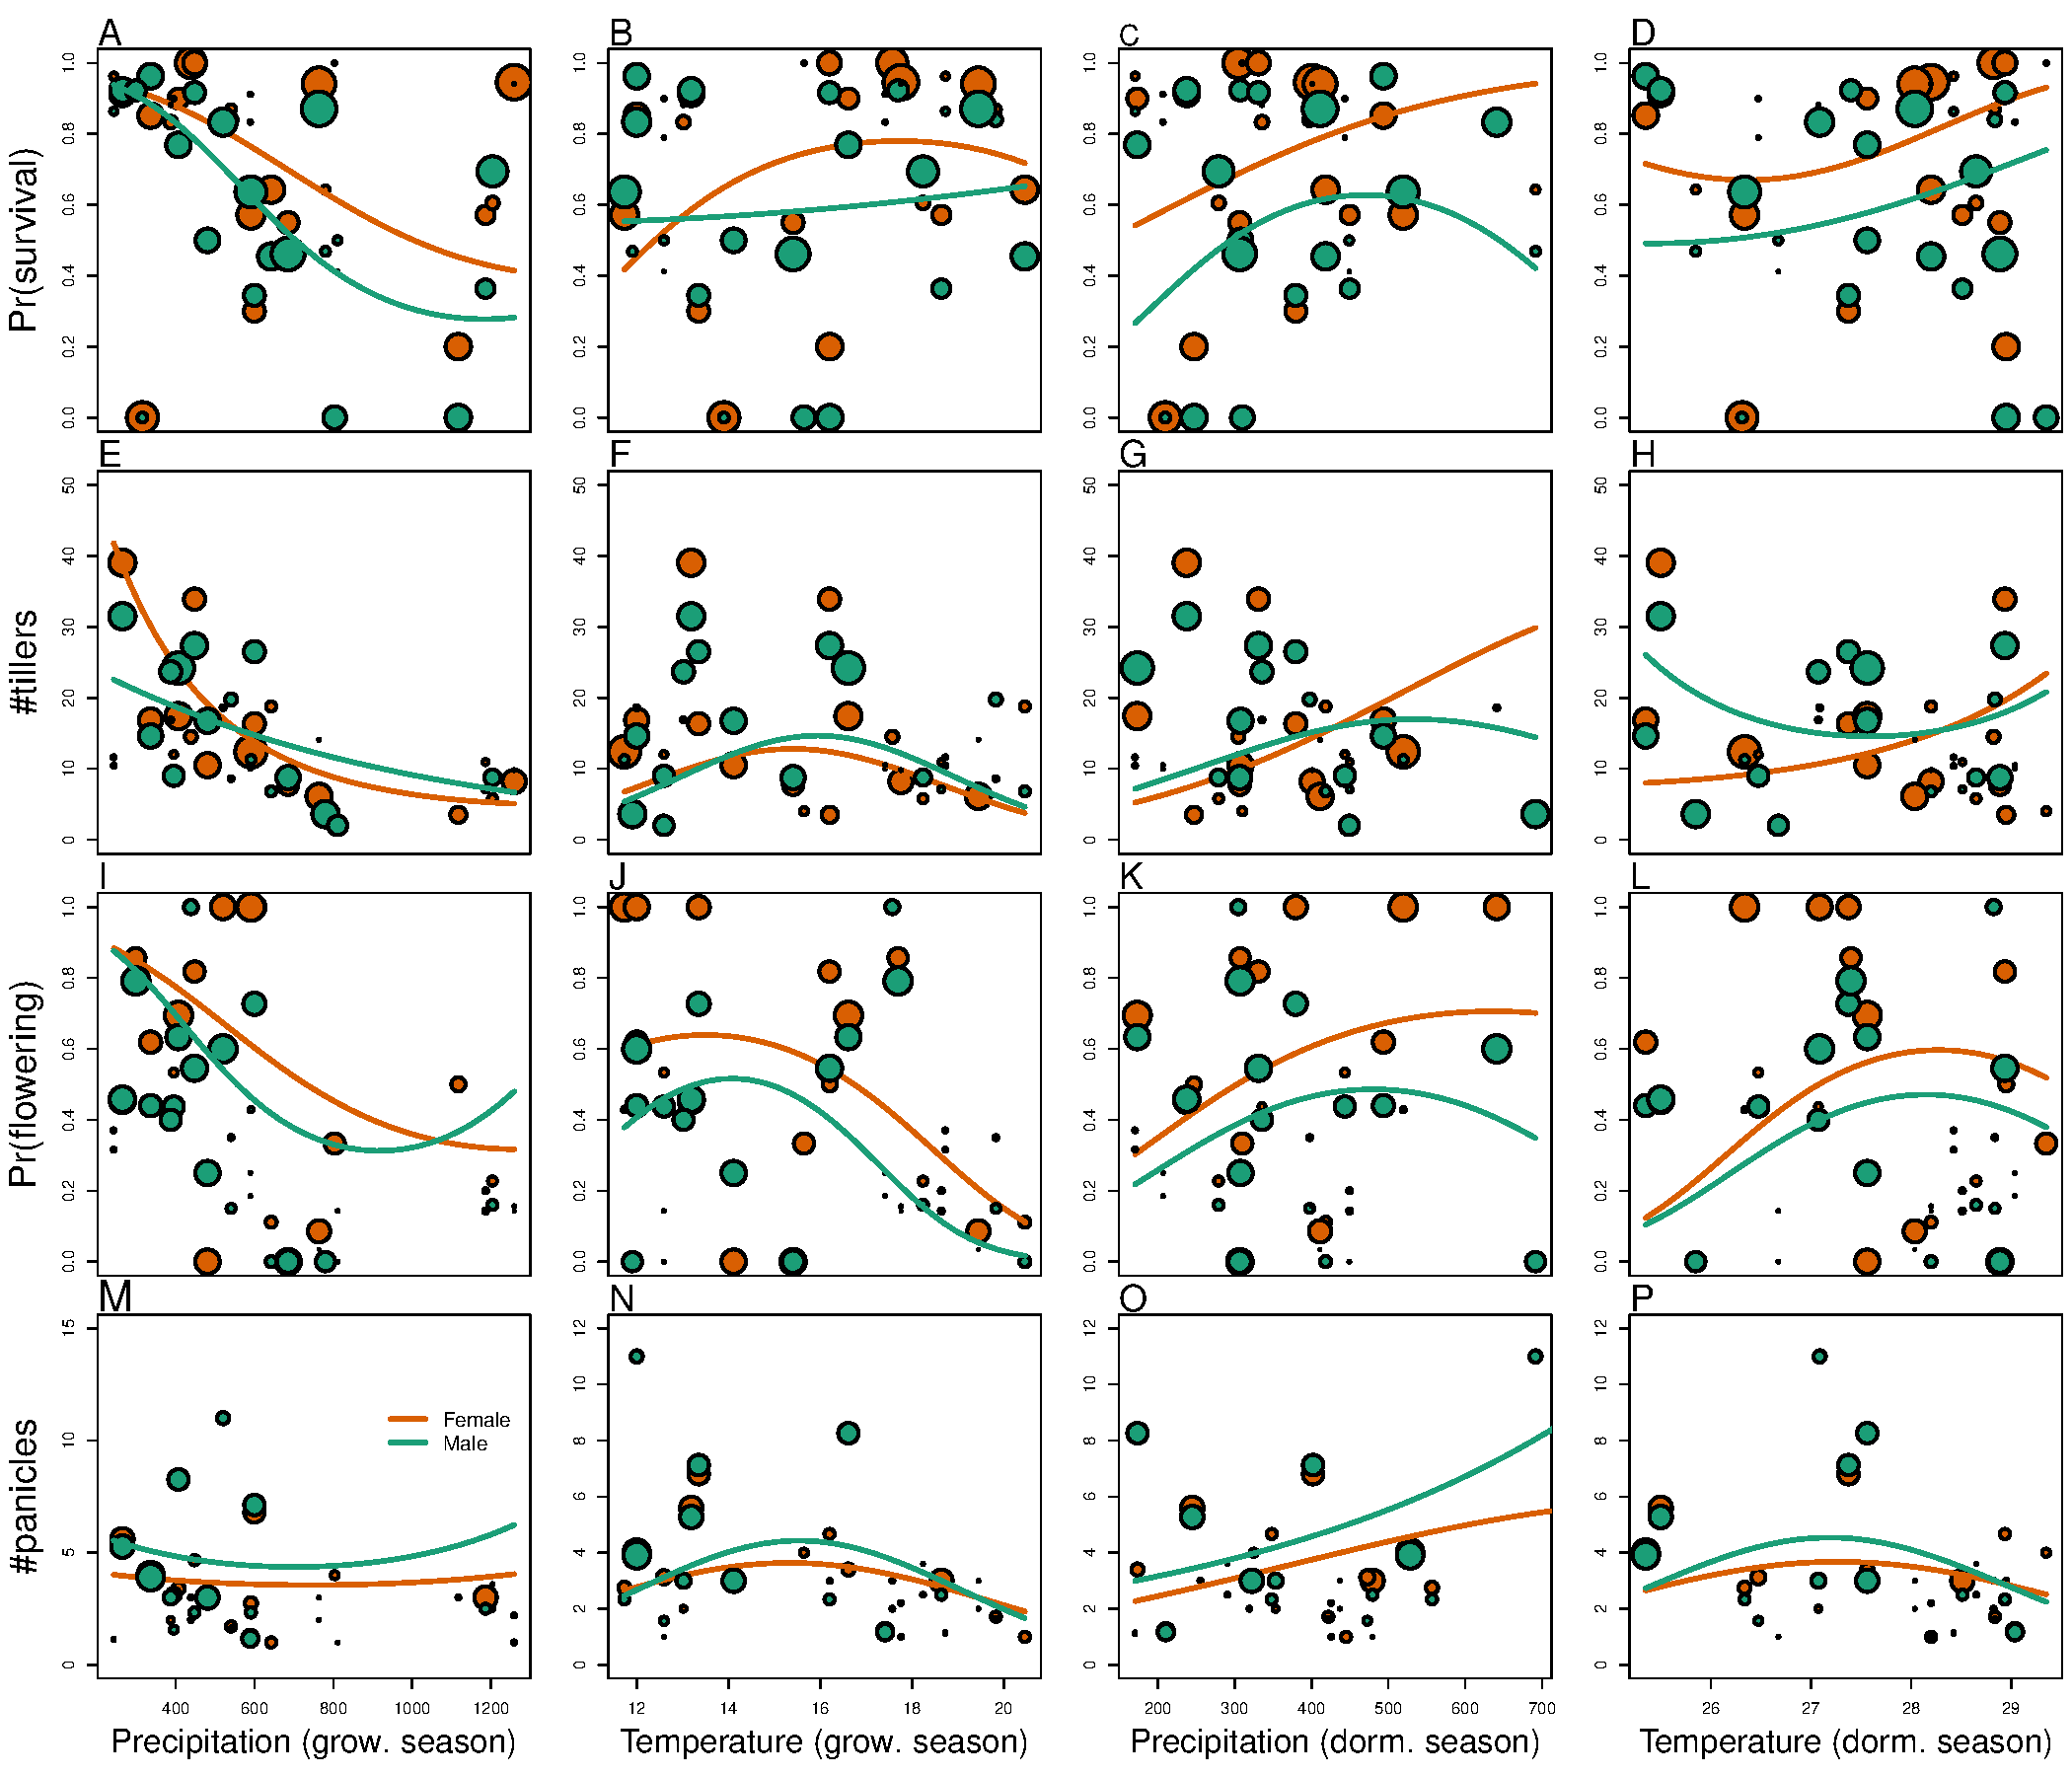
\includegraphics[width=0.95\linewidth]{Figures/vital_rates_v1.pdf}
		\caption{\textbf{Sex specific demographic response to climate across species range}.
			% Vital rates as a function of each climatic variable given 3 others climate variables are constant.
			(A, B, C, D) Probability of survival as a function of precipitation and temperature of the growing and dormant season.
			% (C, D) Probability of survival during the dormant season conditional of climate average during the growing season.
			(E, F, G, H) Change in number of tillers as a function of precipitation and temperature of the growing and dormant season.
			% (F, G) Change in number of tillers during the dormant season conditional of climate average during the growing season.
			(I, J, K, L) Probability of flowering as a function of precipitation and temperature of growing and dormant season.
			% (K, L) Probability of flowering during the dormant season conditional of climate average during the growing season.
			(M, N, O, P) Change in number of panicles as a function of precipitation and temperature of the growing and dormant season.
			% (O, P) Change in number of panicles produced given flowering during the dormant season conditional of climate average during the growing season.
			Points show means by site for females (orange) and males (green). 
			Points sizes are proportional to the sample sizes of the mean and are jittered.
			Lines show fitted statistical models for females (orange) and males (green) based on posterior mean parameter values.
			%Lower panels below each data panel show the posterior distribution of the difference between females and males as a function of climate (positive and negative values indicate female and male advantage, respectively); dashed horizontal line shows zero difference.
			% Statistical results are shown in Figure \ref{Sup:Posterior}.
		}
		\label{fig:vital_rates}
	\end{center}
\end{figure}

Across common garden sites, operational sex ratio (proportion of female panicles) of the experimental populations was female-biased on average ($\approx 60$ \%), reflecting the overall greater rates of female vs. male flowering rather than bias in the underlying population composition (all sites were planted with equal numbers of females and males). 
In addition, across sites and years, OSR  was higher at extreme values of temperature (Figure \ref{Sup:gardens_OSR}, Figure \ref{Sup:posterior_OSR}). 

\subsection*{Climate drivers of population viability across niche space}
Putting all vital rates together in the MPM framework reveals how climate shapes fitness variation across niche dimensions and geographic space, and how accounting for sex structure modifies these inferences. 
Figure \ref{fig:niche} shows the estimated probability of population viability ($\lambda \ge 1$) across seasonal climate niche space; these probabilities account for uncertainty in the vital rate parameters as well as process error related to spatial heterogeneity and genotypic variation. 
For both female-dominant and two-sex models, fitness variation across niche space was dominated by temperature, with weaker effects of precipitation (compare vertical and horizontal contours in Fig. \ref{fig:niche}). 
\tom{These visual trends are supported by LTRE decomposition indicating that variation in fitness across climatic conditions is most strongly driven by responses to growing and dormant season temperature, with weaker interactive effects of precipitation that modulate the effects of temperature (Figure \ref{Sup:LTRE}). 
LTRE analysis also showed that declines in population viability at high and low temperatures were driven most strongly by reductions in vegetative growth and panicle production, with stronger contributions from females than males (Figure \ref{Sup:LTRETemp}). }{You can see here that I am suggesting we moved the lamdba vs climate figure to an appendix. If you disagree we can keep it, but I think the niche space results are the better figure to show.}
Intermediate temperatures of both growing and dormant seasons were associated with near-certain projections of population viability ($Pr(\lambda \ge 1) \approx 1$), and high and low temperature extremes during both seasons were associated with low niche suitability ($Pr(\lambda \ge 1) < 0.2$). 
Higher precipitation slightly expanded the range of suitable temperatures during the dormant season (Fig. \ref{fig:niche}A), and the reverse was true in the growing season (Fig. \ref{fig:niche}B). 
\tom{Points in Fig. \ref{fig:niche} show that climate change forecasted for the common garden locations would move many of them toward lower-suitabiltiy regions of niche space associated with high growing and dormant season temperatures (see also Fig. \ref{fig:lambda_LTRE}).}{I think we should redraw this without countours so that the points are more readable. I would also change the point types and sizes.} 

While the female-dominant and two-sex models were generally in agreement about high confidence in intermediate temperature optima, they differed around the edges of niche space (\tom{Fig. \ref{fig:niche}C,D}{All multi-panel figures need letter labels.},\ref{fig:lambda_LTRE}). 
The female-dominant model over-predicted population viability, especially with respect to growing season temperature. 
For example, the female-dominant model \tom{predicted}{I think I am switching tenses. We will need to clean this up.} that, for most levels of precipitation, warm average growing season (winter) temperatures of $\sim 20\degree C$ had high suitability ($Pr(\lambda \ge 1) > 0.9$), while the two-sex model indicated that these conditions were most likely unsuitable ($Pr(\lambda \ge 1) < 0.5$). 
Similarly, at low winter temperatures that the two-sex model identifies with high certainty as unsuitable ($Pr(\lambda \ge 1) < 0.1$), the female-dominant model is more optimistic ($Pr(\lambda \ge 1) > 0.4$). 
Across growing season climate space, the female-dominant model over-estimates population viability by ca. 10\%, on average (Fig. \ref{fig:niche}D, Fig. \ref{Sup:Niche_overestimation}B). 
The difference between female-dominant and two-sex models was qualitatively similar but weaker in magnitude for niche dimensions of the dormant season (Fig. \ref{fig:niche}C, Fig. \ref{Sup:Niche_overestimation}A). 

Female-dominant and two-sex models diverged most strongly in regions of niche space that favored strongly female-biased operational sex ratios (Fig. WE NEED A FIGURE FOR THIS). 
This suggests mate limitation as the biological mechanism underlying model differences. 
The two-sex model accounts for feedbacks between OSR and female fertility, with reduced seed viability at OSR exceeding $\sim$ 75\% female panicles (Fig. WE NEED A FIGURE FOR THIS).
Lacking this feedback, the female-dominant model over-predicts population viability in regions of niche space where male flowering is not sufficient to maximize seed set. 

\begin{figure}[H]
	\begin{center}
		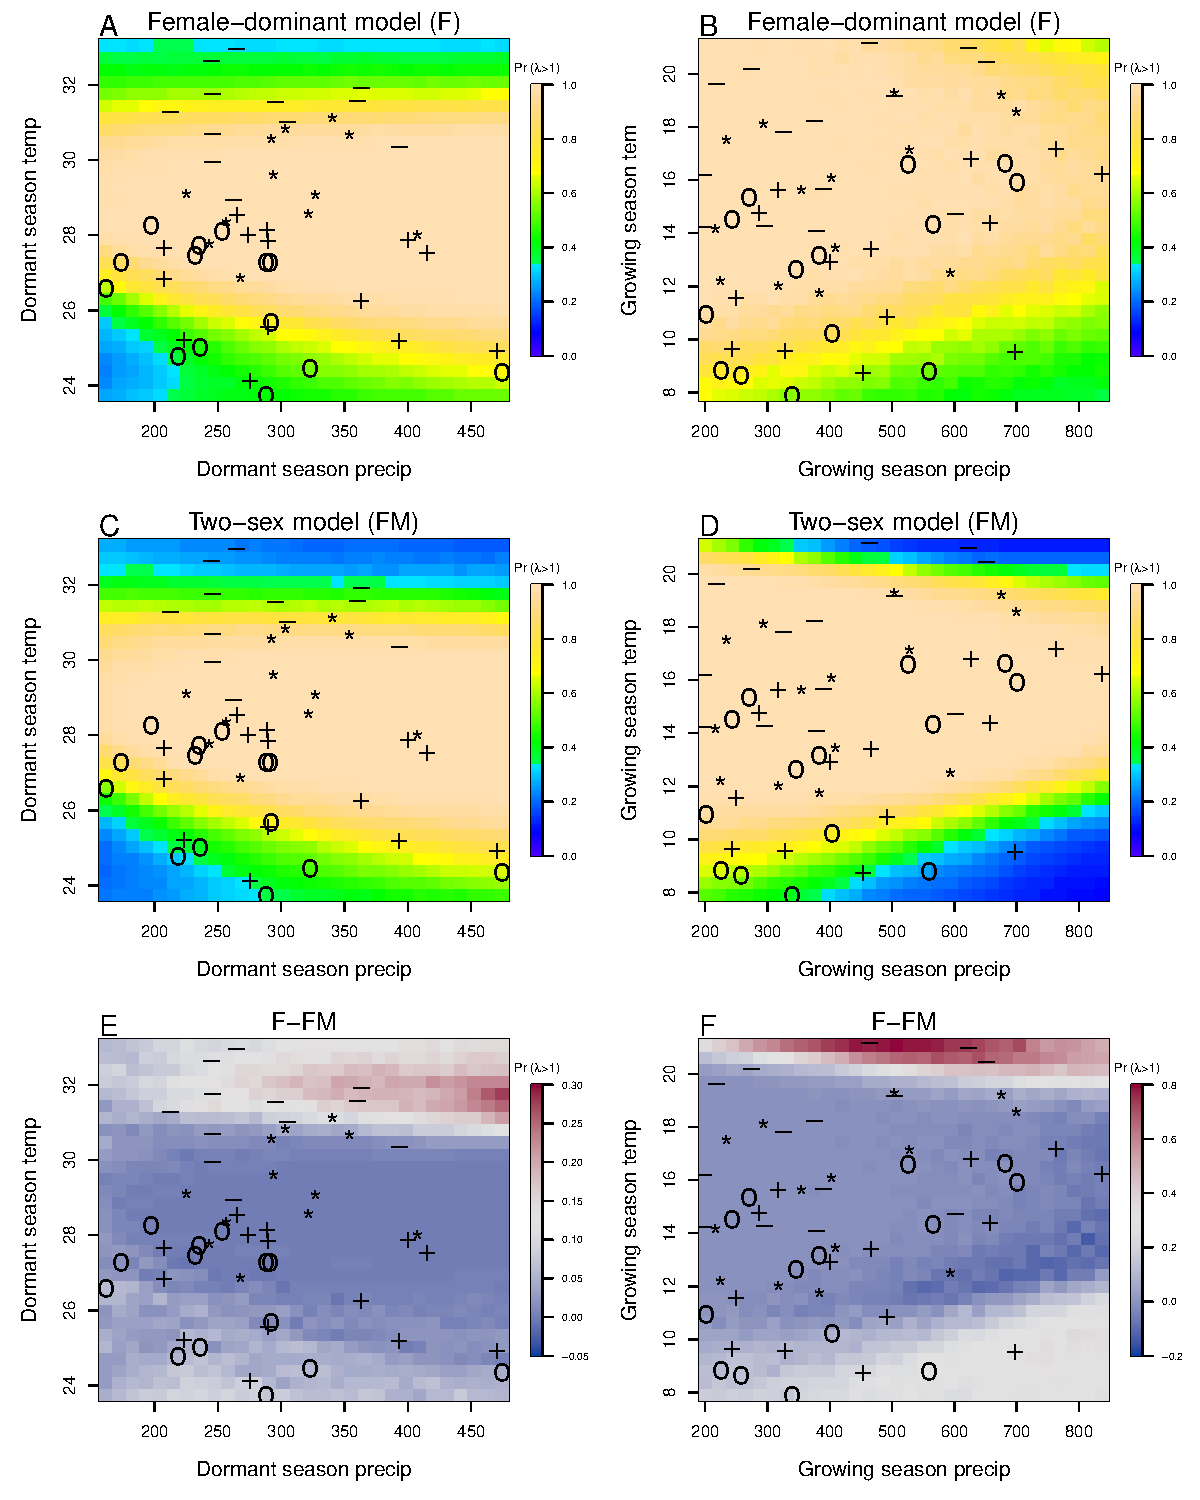
\includegraphics[width=0.95\linewidth]{Figures/niche_dormant_growing.pdf}
		\caption{\textbf{A two‐dimensional representation of the predicted niche shift over time (past, present and future climate conditions)}. 
			%Contours on the first four panels show predicted probabilities of self- sustaining populations, Pr ($\lambda > 1$) conditional on precipitation and temperature of the dormant and growing season.
			% (A) Niche ( Pr ($\lambda$ > 1)) of dormant season for female dominant model, (B) Niche of growing season for female dominant model.
			% (C) Niche ( Pr ($\lambda$ > 1))of dormant season for the two sex model, (B) Niche of growing season for the two-sex model.
			%The last two panels show difference in niche estimation between the female dominant model and the two-sex model for each season.
			"\begin{normalsize}\textbf{o}\end{normalsize}": Past, "\begin{normalsize}\textbf{+}\end{normalsize}": Current,"\begin{large}\textbf{*}\end{large}": RCP 4.5,"\begin{large}\textbf{-}\end{large}": RCP 8.5.
			}
		\label{fig:niche}
	\end{center}
\end{figure}

\subsection*{Climatic change induces shifts in geographic niche and population OSR}
Projecting the climatic niche onto geographic space, we find that suitable niche conditions for Texas bluegrass are shifting north under climate change (Fig. \ref{fig:geoprojcmc}). 
Under past (1901-1930) and present (1990-2019) conditions, the two-sex and female-dominant models predict widespread suitability with high confidence ($Pr(\lambda \ge 1) \approx 1$) across much of Texas and Oklahoma. 
For both models, the predicted geographic niche generally corresponds well to independent observations of the Texas bluegrass distribution (Fig. \ref{fig:geoprojcmc}).
The predicted geographic niche is more expansive than the observed distribution, particularly at southern, western, and eastern edges, suggesting some degree of range disequilibrium (e.g., due to dispersal limitation), geographic bias in occurrence observations, and/or model mis-specification. 
Comparing past to present conditions, the geographic niche for both models has shifted slightly poleward, with reductions in viability at the southern margins and expansions of viability at northern margins. 
The northward shift of suitable niche conditions is even more pronounced in projections to end-of-century (2071-2100) conditions, with the most dramatic changes in the most pessimistic (RCP8.5) scenario (\jacob{Fig. \ref{fig:geoprojcmc}.}{I am not sure if we need title for each panel. }). 
In fact, under the pessimistic scenario, Texas bluegrass will have very little remaining climate suitability in the state of Texas by the end of the 21st century. 
The predicted poleward niche shift is consistent across different global circulation models (Figure \ref{Sup:geoprojces}, Figure \ref{Sup:geoprojacc}, Figure \ref{Sup:geoprojmiroc}). 

Female-dominant and two-sex models are in broad agreement about northward migration of the climatic niche, but the geographic projections reveal hotspots of disagreement where the female-dominant model over-predicts climate suitability and under-predicts the likelihood of range shifts (Fig. \ref{fig:geoprojacc}). 
These hotspots are generally regions of predicted female bias in the operational sex ratio (Fig. WE NEED A FIGURE FOR THIS.) 
The strongest contrast between the two models is in the pessimistic climate change scenario (RCP8.5), where the female-dominant model over-predicts population viability by \tom{ca. 25\%}{I just eyeballed this. Real number should come from the histograms.} across much of the region (Figure \ref{Sup:geo_overestimation}) and under-estimates the magnitude of a potential range shift. 
In this scenario, a broad swath of the current distribution that is forecasted to by effectively unsuitable ($Pr(\lambda \ge 1) \approx 0$) by the two-sex model is identified as marginally suitable ($Pr(\lambda \ge 1) \approx 0.5$) by the female-dominant model. 
Accordingly, the OSR of Texas bluegrass across its range is projected to be ca. 75\% female panicles, on average, by end of century under RCP8.5, an increase from ca. 60\% female under projections for past and current conditions (Fig. \ref{fig:srprojcmc}). 
The more optimistic climate change scenario (RCP4.5) predicts an intermediate shift in OSR, with hotspots of change becoming strongly female-biased but most of the range remaining near current levels of 60\% female (Fig. \ref{fig:srprojcmc}; WE NEED A MAP SHOWING WHERE OSR IS BECOMING MORE BIASED). 

\begin{figure}[H]
	\begin{center}
		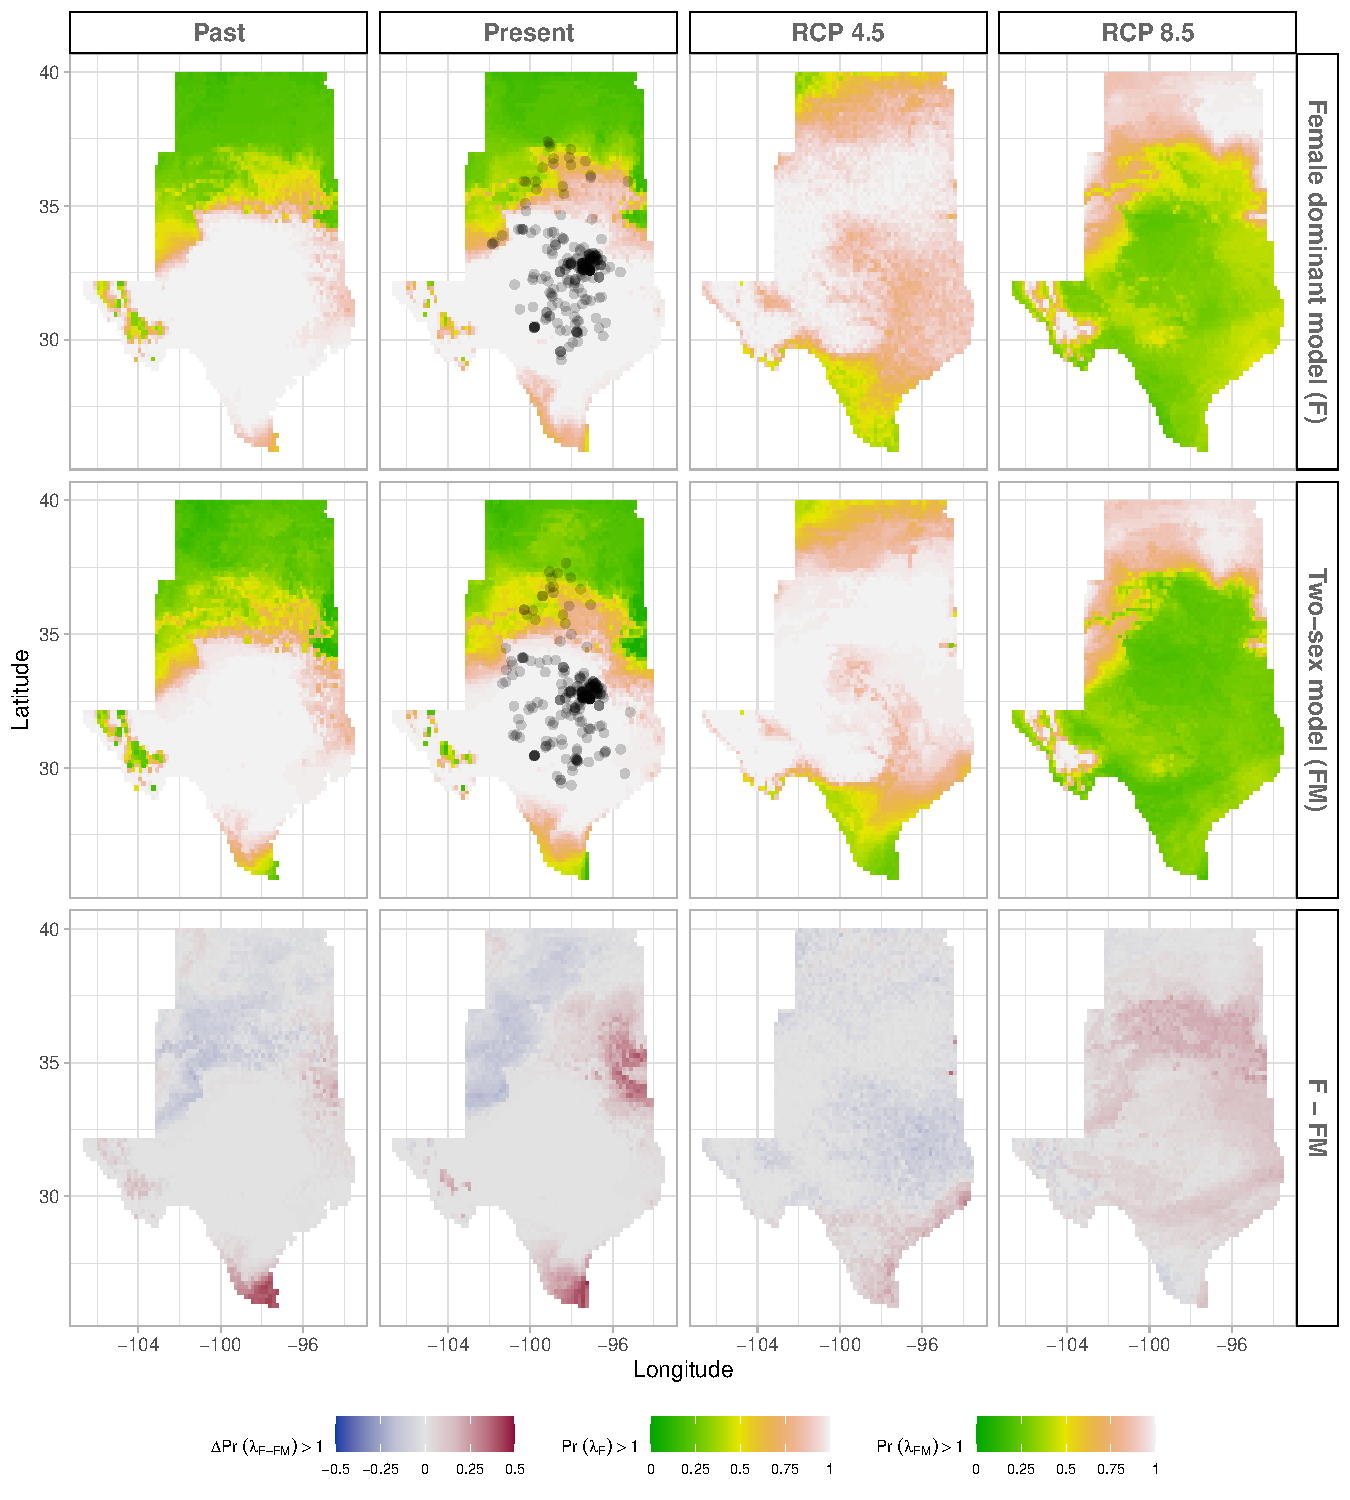
\includegraphics[width=0.99\linewidth]{Figures/Fig_geoPrlambdacmc.pdf}
		\caption{ \textbf{Climate change favors range shift towards north edge.}
			(A) Past, (B) Current, (C and D) Future predicted range shift based on the predicted probabilities of self- sustaining populations, Pr ($\lambda > 1$), using the two-sex model that incorporates sex- specific demographic responses to climate with sex ratio dependent seed fertilization.
			(E) Past, (F) Current, (G and F) Future  predicted range shift based on the predicted probabilities of self- sustaining populations, Pr ($\lambda > 1$), using the female dominant model.
			Future projections were based on the CMCC-CM model.
			The black dots on panel B and F indicate all known presence points collected from GBIF. 
			The occurrences of GBIFs are distributed in with higher population fitness habitat Pr ($\lambda$ > 1) , confirming that our study approach can reasonably predict range shifts. }
		\label{fig:geoprojcmc}
	\end{center}
\end{figure}

\begin{figure}[H]
	\begin{center}
		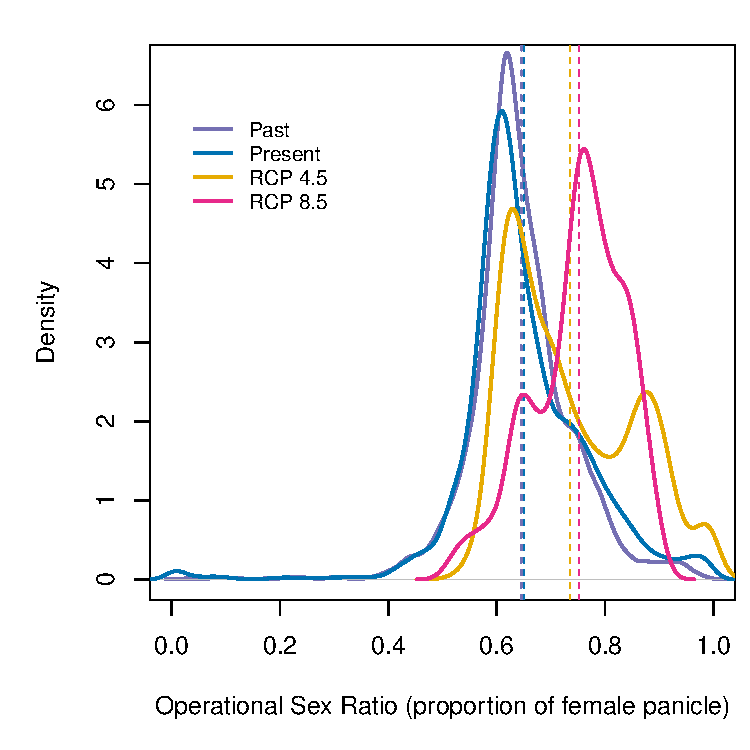
\includegraphics[width=0.7\linewidth]{Figures/POAR_OSR.pdf}
		\caption{Change in Operational Sex Ratio (proportion of female panicle) over time (past, present, future).
			Future projections were based on the CMCC-CM model.
			The mean sex ratio for each time period is shown as vertical dashed line.}
		\label{fig:srprojcmc}
	\end{center}
\end{figure}

\section*{Discussion}
\tom{Dioecious species make up a large fraction of Earth's biodiversity -- most animals and many plants -- yet we have little knowledge about how sex-specific demography and responses to climate drivers may affect population viability and range shifts of dioecious species under climate change.}{Love this opening sentence.}
We used demographic data collected common garden experiments and sex-structured demographic modeling to forecast for the first time the likely impact of climate change on range dynamics of a dioecious species.
% Our models captures a certain range of demographic and environmental variability (Figure \ref{Sup:lambda2sex}).
\tom{Our future projections require extrapolation to warmer or colder conditions than observed in our experiment and subsequently should be interpreted with caution \citep{chen2024influence}.}{I think extrapolation should be its own paragraph. This also relates to uncertainty in the climate forecasts.}
%Despite all these limitations, the qualitative implications of the response of our study species to increase temperature (dormant and growing season) seems consistent across all GCMs (Figure \ref{Sup:geoprojces}, Figure \ref{Sup:geoprojcmc}, Figure \ref{Sup:geoprojmiroc}).  
% Most of the suitable areas move toward the North, beyond the current range in response to climate change.
% \tom{Climate change will affect population growth rate primarily through the response of female which is more sensitive to climate change \citep{miller2022two}.}{This paper says the opposite.}
% \tom{Males also have a significant contribution to population growth rate particularly for temperature. }{I do not know what this is saying.}
Three general patterns emerged from our analysis of range-wide common garden experiments and sex-structured, climate-explicit demographic models.
First, our Bayesian mixed effect model suggests a sex specific demographic response to climate change that lead to higher proportion of female as climate increase.
Second, climate change favors a northern range shifts in suitable  habitats. 
Third, the female dominant model (model that does not account for sex structure) overestimates species niche and range shifts.

There was a female demographic advantage leading to a female biased in response to climate change in \emph{Poa arachnifera} populations.
% The female demographic advantage is not unique to our study system and has been observed in several dioecious species \citep{welbergen2008climate,zhao2012sex,sasaki2019complex}.
The extreme female-bias in response to climate change contrast with  previous studies suggesting that an increase in male frequency in response in climate change \citep{petry2016sex,hultine2016climate}.
Two mechanisms could explain the observed demographic advantage of females over males for survival and flowering and the opposite for growth and number of panicles.
The trade-off between fitness traits (survival, growth and fertility) due to resource limitation and the pollination mode of our study species (wind pollinated) could explain such a result \citep{cipollini1994sexual,freeman1976differential}.
For most species, the cost of reproduction is often higher for females than males due to the requirement to develop seeds and fruits \citep{hultine2016climate}. 
However, several studies reported a higher cost of reproduction for males in wind pollinated species due to the larger amounts of pollen they produce \citep{burli2022environmental,cipollini1994sexual,bruijning2017surviving,field2013comparative}.

% \tom{Under current conditions, most populations across the range are viable.}{I don't think this statement is well-supported. We don't have any data from natural populations.}
% This result could be explained by two hypotheses.
% First, demographic compensation whereby an increase of one vital rate is coupled with a decrease of another vital rate could explain viable populations in harsh conditions at the range edge \citep{doak2010demographic,villellas2015demographic,nomoto2021drivers}. 
% In our system, a decrease in fertility and survival rate was counterbalanced by an increase in flowering rate, \tom{preventing the population growth rate from declining even at range edge}{Not sure I follow this - if lambda was not declining it would not be a range edge} \tom{during the dormant season}{Population growth rate is an annual measure, it does not refer to any season. I think what you mean here is that dormant season weather can affect population growth rate.}.
% Second, local adaptation at the edge of the range could explain the viable populations throughout the range \citep{miller2022two}. 
% \tom{Our study was based on a common garden experiment; therefore, individuals planted in climatic conditions that are similar to their source populations climatic conditions were less impacted by stressful environmental conditions.}{This statement lacks evidence.}
% \tom{An important question to ask is: what is the role of local adaptation in buffering species response against climate change.
% Unfortunately, our model does not shed light on that question.
% Adding another predictor to our complex model would have lead to overfitting. 
% Therefore, the role of local adaptation in mitigating population response to climate should be the next step in forecasting species response to climate. }{I don't think this is a very effective use of the Discussion. If you want to address local adaptation maybe that can go in an appendix. I don't actually understand the point of this paragraph but maybe I am not understanding something.}

% Our LTRE analysis reveals that a small change in temperature of the growing and dormant season could have a larger  impact on population viability.
% % This results corroborated with other studies and suggest that projected future climate will affect population viability \citep{reed2021climate}. 
% Temperature can impact plant populations through different mechanisms. 
% Increasing temperature could increase evaporative demand, affect plant phenology \citep{mclean2016predicting,sherry2007divergence,iler2019reproductive}, and germination rate \citep{reed2021climate}.
% % In the  growing season, when the temperature is high, the effect on the water balance should be strong .
% The potential for temperature to influence these different processes changes seasonally \citep{konapala2020climate}.
% For example, studies suggested that species that are active during the growing season such as cool grass species can have delayed phenology in response to global warming, particularly if temperatures rise above their physiological tolerances \citep{cleland2007shifting,williams2015life}. 
% In addition, high temperature during the growing season by affecting pollen viability, fertilization could affect seed formation and germination \citep{hatfield2015temperature,sletvold2015climate}. 
% % Because our study species was sensitive to temperatures in the growing season, the former mechanism deserve further attention.
% \tom{Temperature also affected operational sex ratio (OSR) (Fig.XX). 
% That variation in OSR could affect population growth rate by altering females’ fitness \citep{petry2016sex,knight2005pollen,haridas2014frequency}. }{These results need to be beter developed because they underlie all the other results. And again, the only way you can get an effect on temperature on OSR is if there were sex-specific responses to climate, but you way there were none.}

Our results suggest that climate change will alter population at the center of the range and drive a northern range shifts. 
This impact of climate change on the species current niche could be explained by the increase of temperature over the next years.
Small change in temperature of the growing and dormant season have a larger impact on population viability.
Temperature can impact plant populations through different mechanisms.
Increasing temperature could increase evaporative demand, affect plant phenology \citep{mclean2016predicting,sherry2007divergence,iler2019reproductive}, and germination rate \citep{reed2021climate}.
% In the  growing season, when the temperature is high, the effect on the water balance should be strong .
The potential for temperature to influence these different processes changes seasonally \citep{konapala2020climate}.
For example, studies suggested that species that are active during the growing season such as cool grass species can have delayed phenology in response to global warming, particularly if temperatures rise above their physiological tolerances \citep{cleland2007shifting, williams2015life}.
In addition, high temperature during the growing season by affecting pollen viability, fertilization could affect seed formation and germination \citep{hatfield2015temperature,sletvold2015climate}.
Pollen dispersal may allow plants to resist climate change because pollen dispersal may provide the local genetic diversity necessary to adapt at the leading edge of the population \citep{kremer2012long,corlett2013will,duputie2012genetic}.
Since wind pollination is most effective at short distances, it is most often found in plant species growing at high density such as our study species, it is less likely that dispersal limitation  affect niche shift in our study system.
Difference in non-climatic factors such as soil, or biotic interactions could also explain decline in population growth rate as an indirect effects of increase in temperature \citep{alexander2015novel,schultz2022climate}.
For example, climate change could increase the strength of species competition and thereby constrain our study species  to a narrower realized niche \citep{pulliam2000relationship,aguilee2016pollen}.
% Future studies should studies should investigate how biotic factors drive range limits. 

We found evidence of underestimation of the impact of climatic change on population dynamics by the female dominant model and implication for such an underestimation on conservation actions for dioecious species.
The underestimation of the impact of climatic change on population dynamics by the female dominant model makes sense given the sex specific response to climatic change. 
\emph{Poa arachnifera} populations will be female biased in response to climate change.
That extreme female-bias could affect population growth rate by altering males’ fitness with reduction on mate availability given that females individuals have a demographic advantage over males \citep{knight2005pollen,haridas2014frequency}.
Further, our work suggest that population viability is sensitive to climate under current  and future conditions.
This is key because most conservation actions are design from  data on current responses to climate, rather than future response to climate \citep{sletvold2013climate}.
Since the role of male is not negligible in accuraltly predicting dioecious species response to climate change, management strategies that focus on both sexes would be effective and will enhance our understanding of dioecious species response to global warming.

\section*{Conclusion}
We have investigated the potential consequence of skewness in sex ratio on population dynamics and range shift in the context of climate change using the Texas bluegrass. 
We found extreme female -biased in response to climate change. 
The effect of female biased will induce range shifts to the northern edge of the species current range by limiting mate availability.
Beyond, our study case, our results also suggest that tracking only one sex could lead to an underestimation of the effect of climate change on population dynamics. 
Our work  provides also a framework for predicting the impact of global warming on population dynamics using the probability of population to self-sustain. 

\section*{Acknowledgements}
This research was supported by National Science Foundation Division of Environmental Biology awards 2208857 and 2225027. 
We thank the institutions who hosted us at their field station facilities, including

\newpage
\bibliographystyle{apalike}
\bibliography{Forecasting}

%--------------------------------------------------------------------
\newpage
\clearpage 
\setcounter{equation}{0}
\setcounter{figure}{0}
\setcounter{section}{0}
\setcounter{table}{0}
\renewcommand{\theequation}{S.\arabic{equation}}
\renewcommand{\thetable}{S-\arabic{table}}
\renewcommand{\thefigure}{S-\arabic{figure}}
\renewcommand{\thesection}{S.\arabic{section}}

\centerline{\Large{\textbf{Supporting Information}}}



\section {Supporting Figures}

\begin{figure}[H]
	\centering
	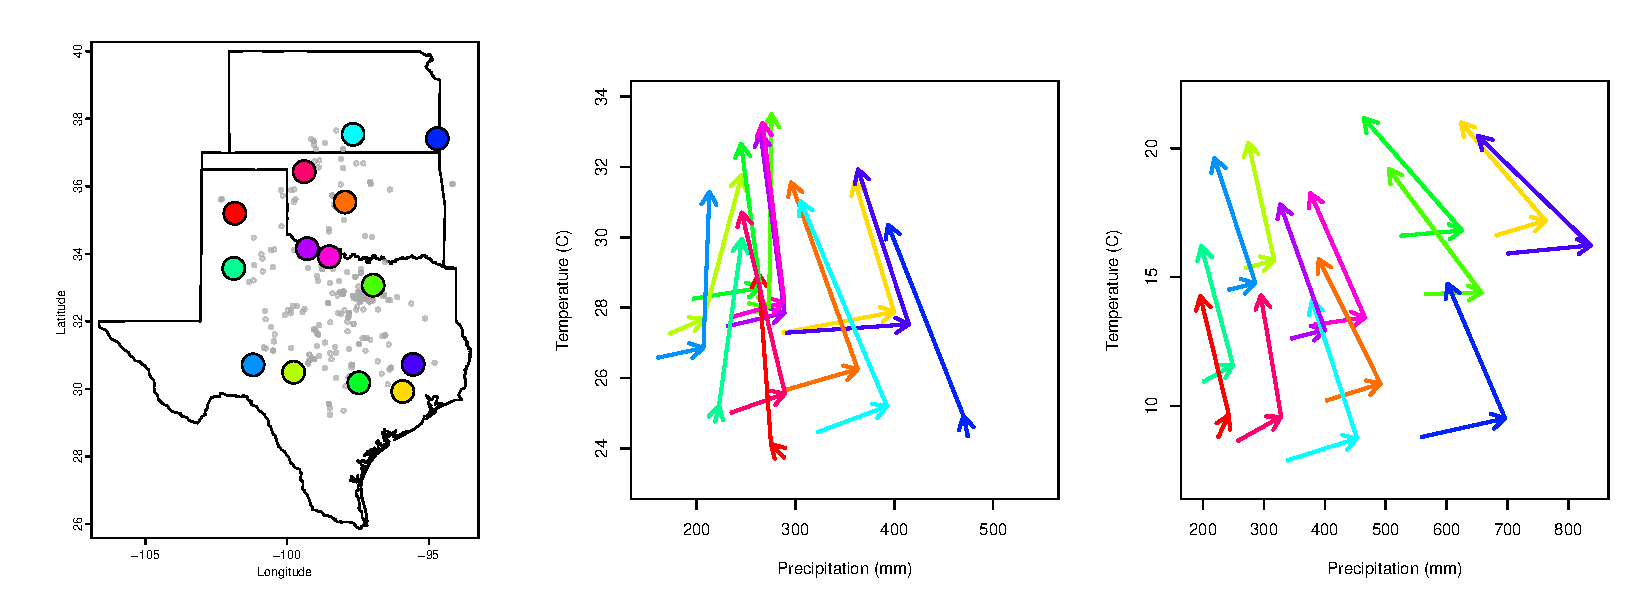
\includegraphics[width=0.959\linewidth]{Figures/tom_map_v1.pdf}
	\caption{(A), Common garden locations in Texas, Oklahoma, and Kansas (points) and (B,C) corresponding changes in growing and dormant season climate. Arrows in B,C connect past (1901-1930) and present (1990-2019) climate normals, and present and future (2071-2100) climate normals under RCP4.5 and RCP8.5 forecasts. Future forecasts are from MIROC5 but other climate models show similar patterns.}
	\label{Sup:climate_variation1}
\end{figure}

%\begin{figure}[H]
%	\centering
%	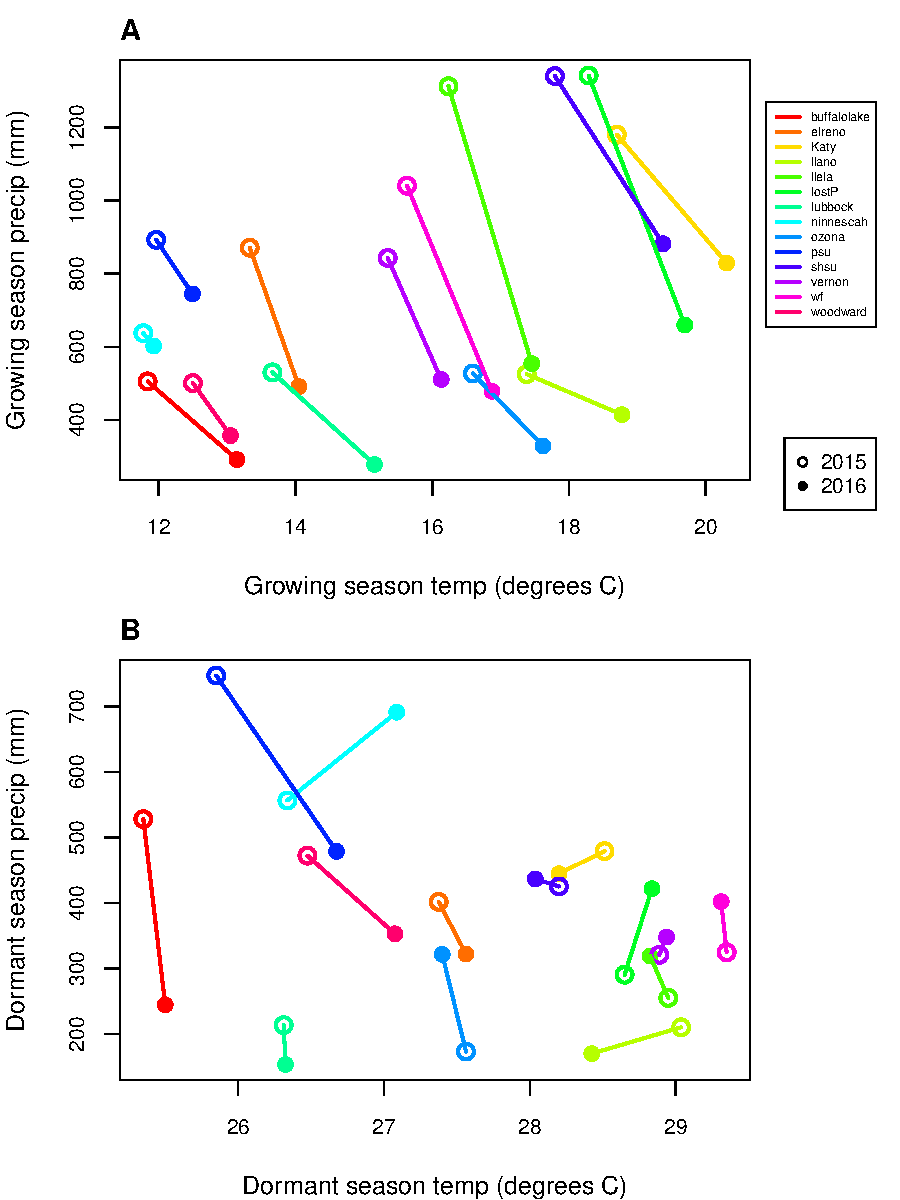
\includegraphics[width=0.959\linewidth]{Figures/site_year_weather.pdf}
%	\caption{Seasonal climate variation (temperature in \degree C and precipitation in $mm$) across the common garden sites during the 2014--15 and 2015--16 census years. Each color represents a site and lines connect the same site between years.}
%	\label{Sup:climate_variation2}
%\end{figure}

\begin{figure}[H]
	\centering
	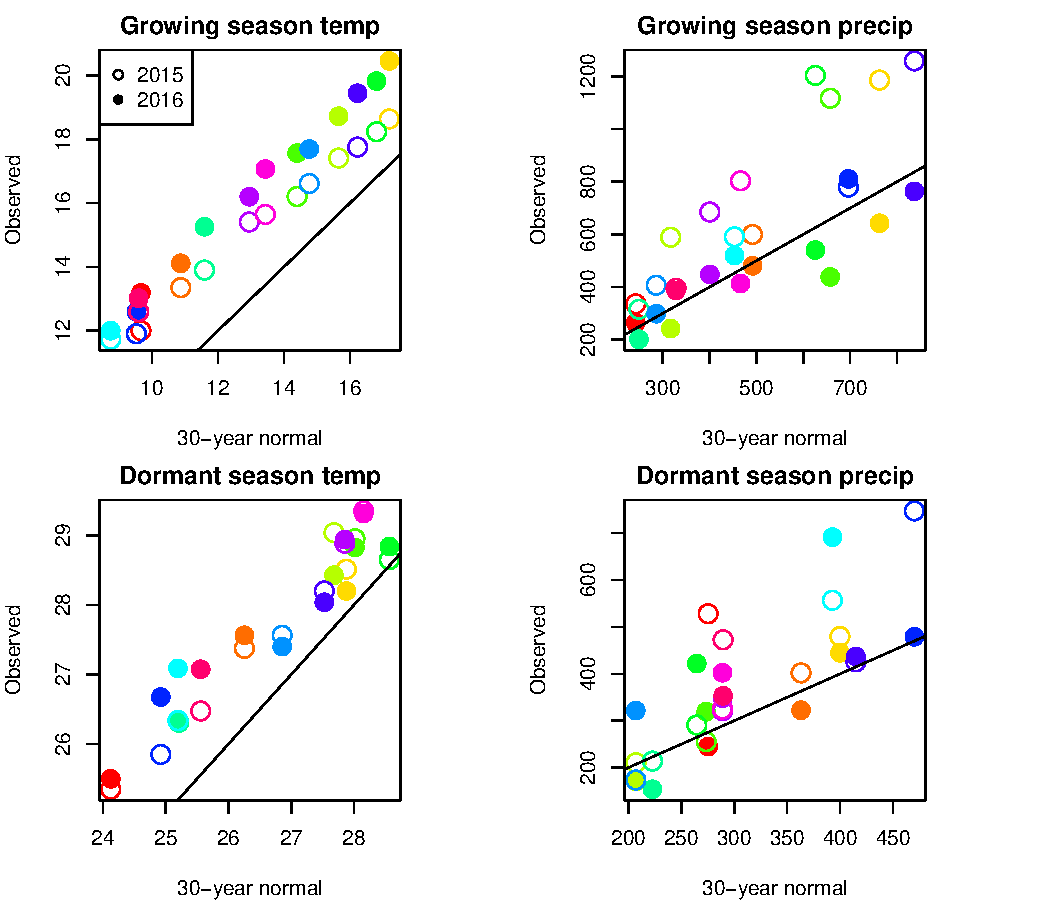
\includegraphics[width=0.959\linewidth]{Figures/clim_norm_vs_weather.pdf}
	\caption{Comparison of 30-year (1990-2019) climate normals and observed weather conditions at common garden sites during the 2014--15 and 2015--16 census periods. Temperature is in \degree C and precipitation is in $mm$. Colors represent sites and lines show the $y=x$ relationship.}
	\label{Sup:climate_normal_weather}
\end{figure}

\begin{figure}[H]
	\centering
	\includegraphics[width=0.75\linewidth]{Figures/PPC.pdf}
	\caption{Posterior predictive checks. Consistency between real data and simulated values suggests that the fitted vital rate models accurately describes the data. Graph shows density curves for the observed data (light orange ) along with the simulated values (dark orange).}
	\label{Sup:PPC}
\end{figure}

\begin{figure}[H]
	\centering
	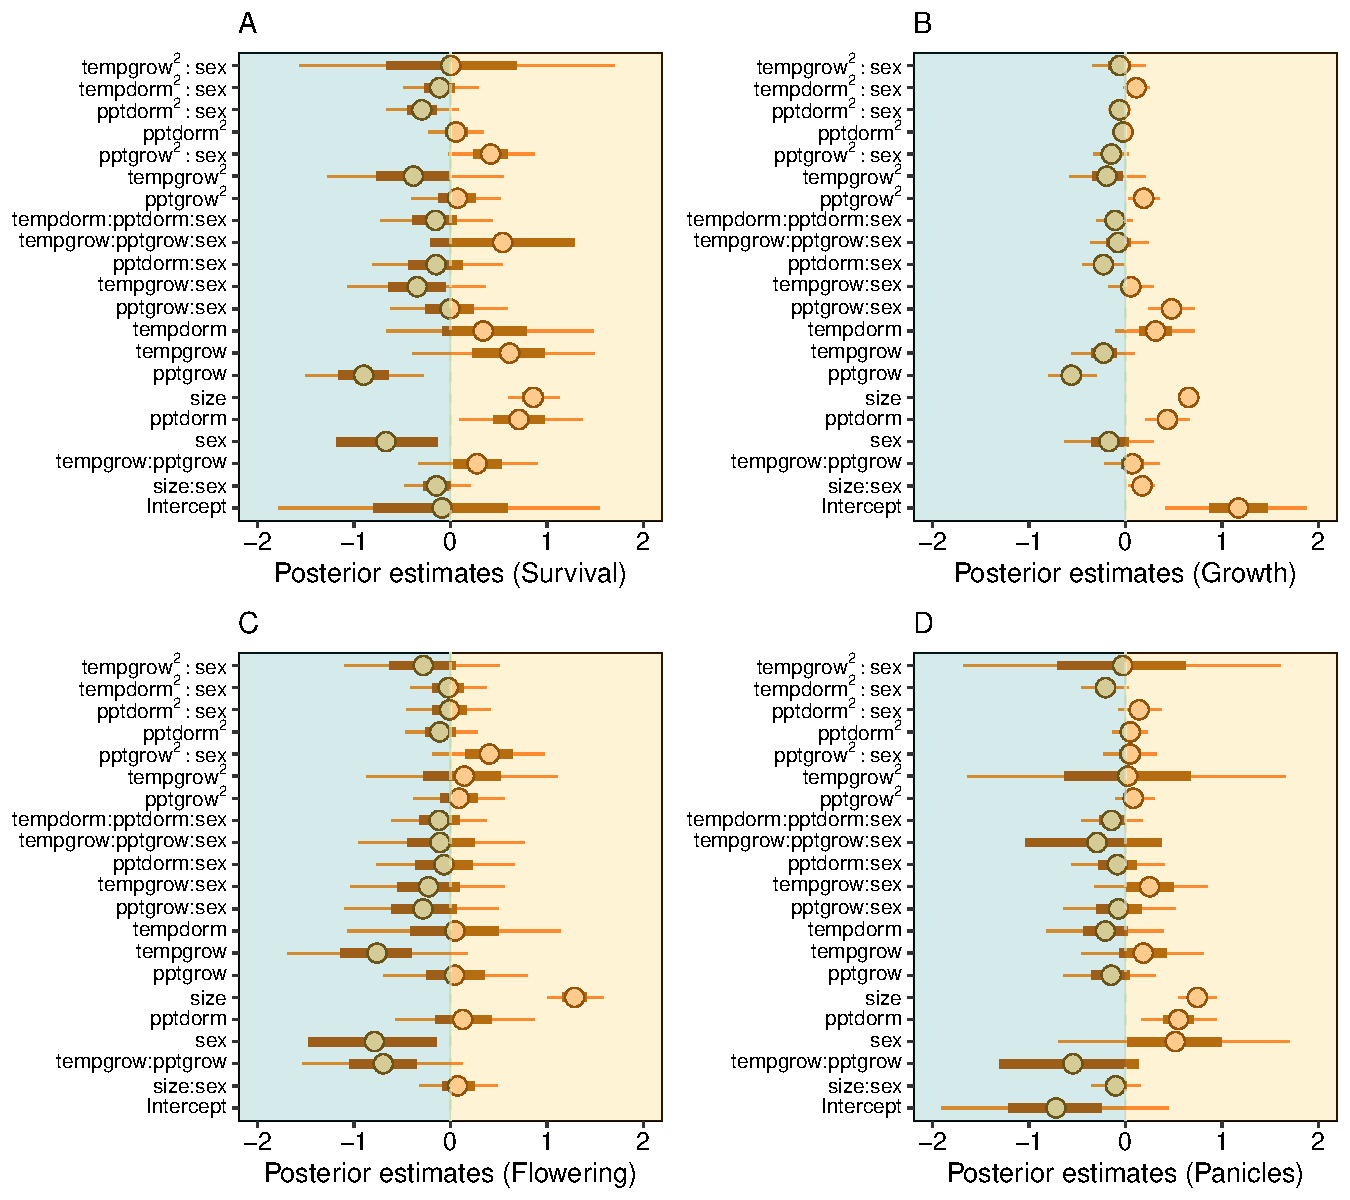
\includegraphics[width=0.99\linewidth]{Figures/Posterior_mean.pdf}
	\caption{Mean parameter values and 95\% credible intervals of the posterior probability distributions. 
		pptgrow is  the precipitation of growing season,
		Tempgrow is the temperature of growing season,
		pptdorm is the temperature of dormant season,
		Tempdorm is the temperature of dormant season.}
	\label{Sup:Posterior}
\end{figure}

\begin{figure}[H]
	\centering
	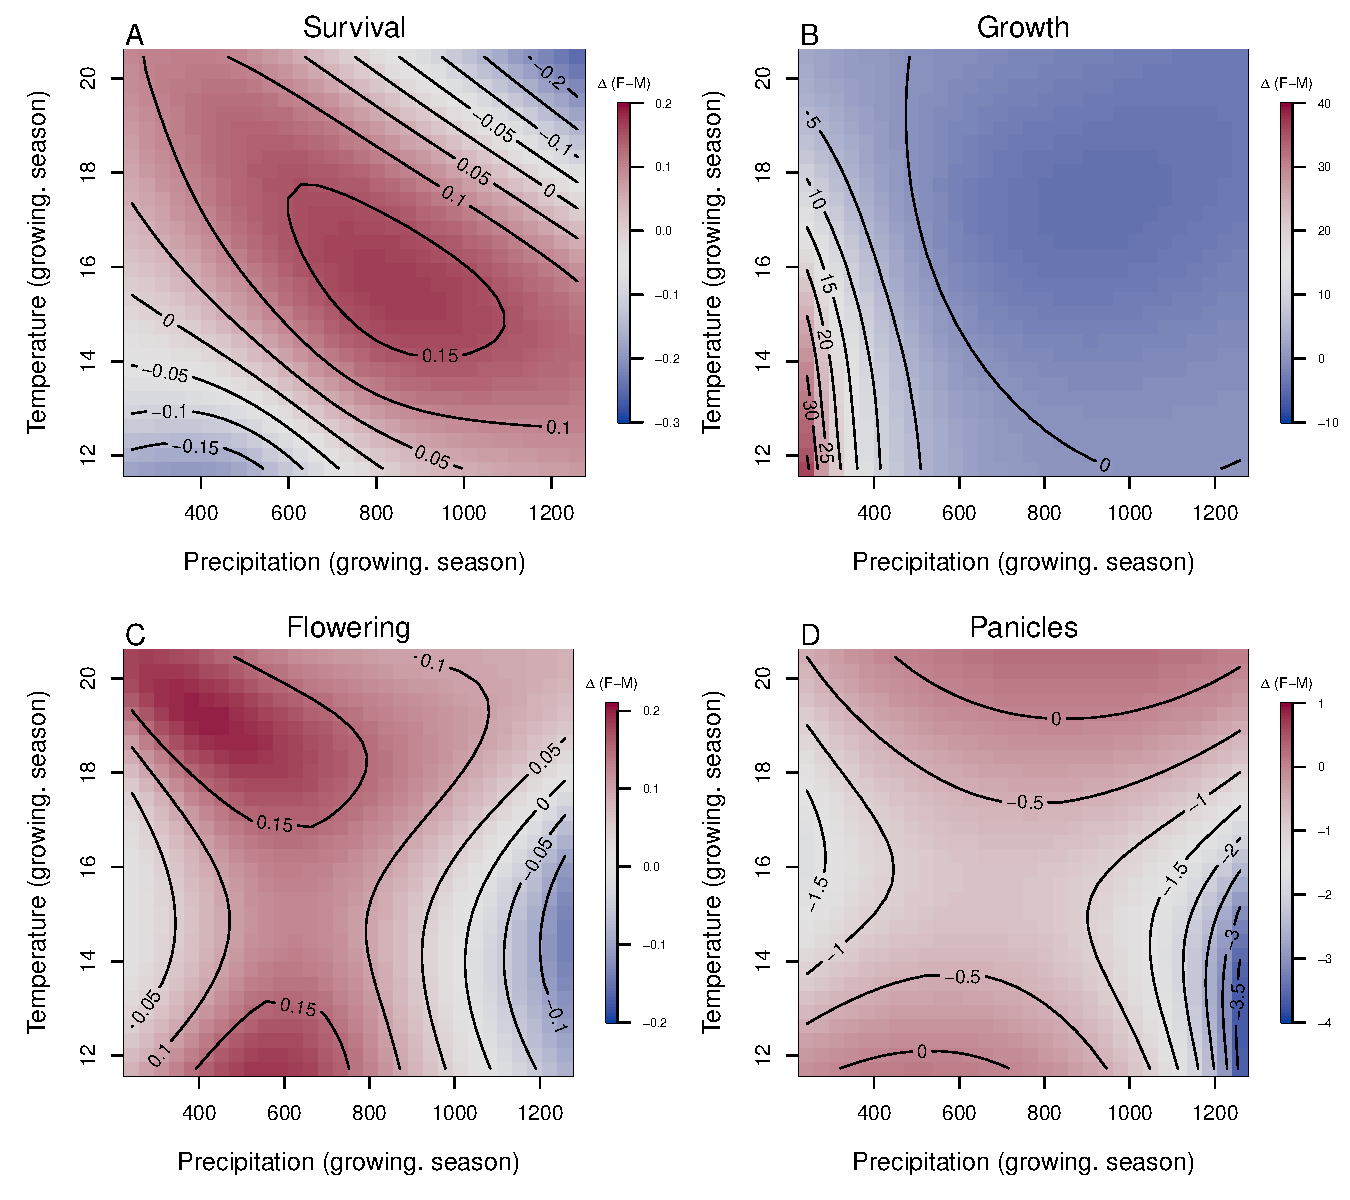
\includegraphics[width=0.99\linewidth]{Figures/Vital_rate_growing_3D.pdf}
	\caption{ Predicted difference in demographic response to climate across species range between female and male. Contours show predicted value of that difference conditional on precipitation and temperature of  growing season }
	\label{Sup:vt_3D_grow}
\end{figure}

\begin{figure}[H]
	\centering
	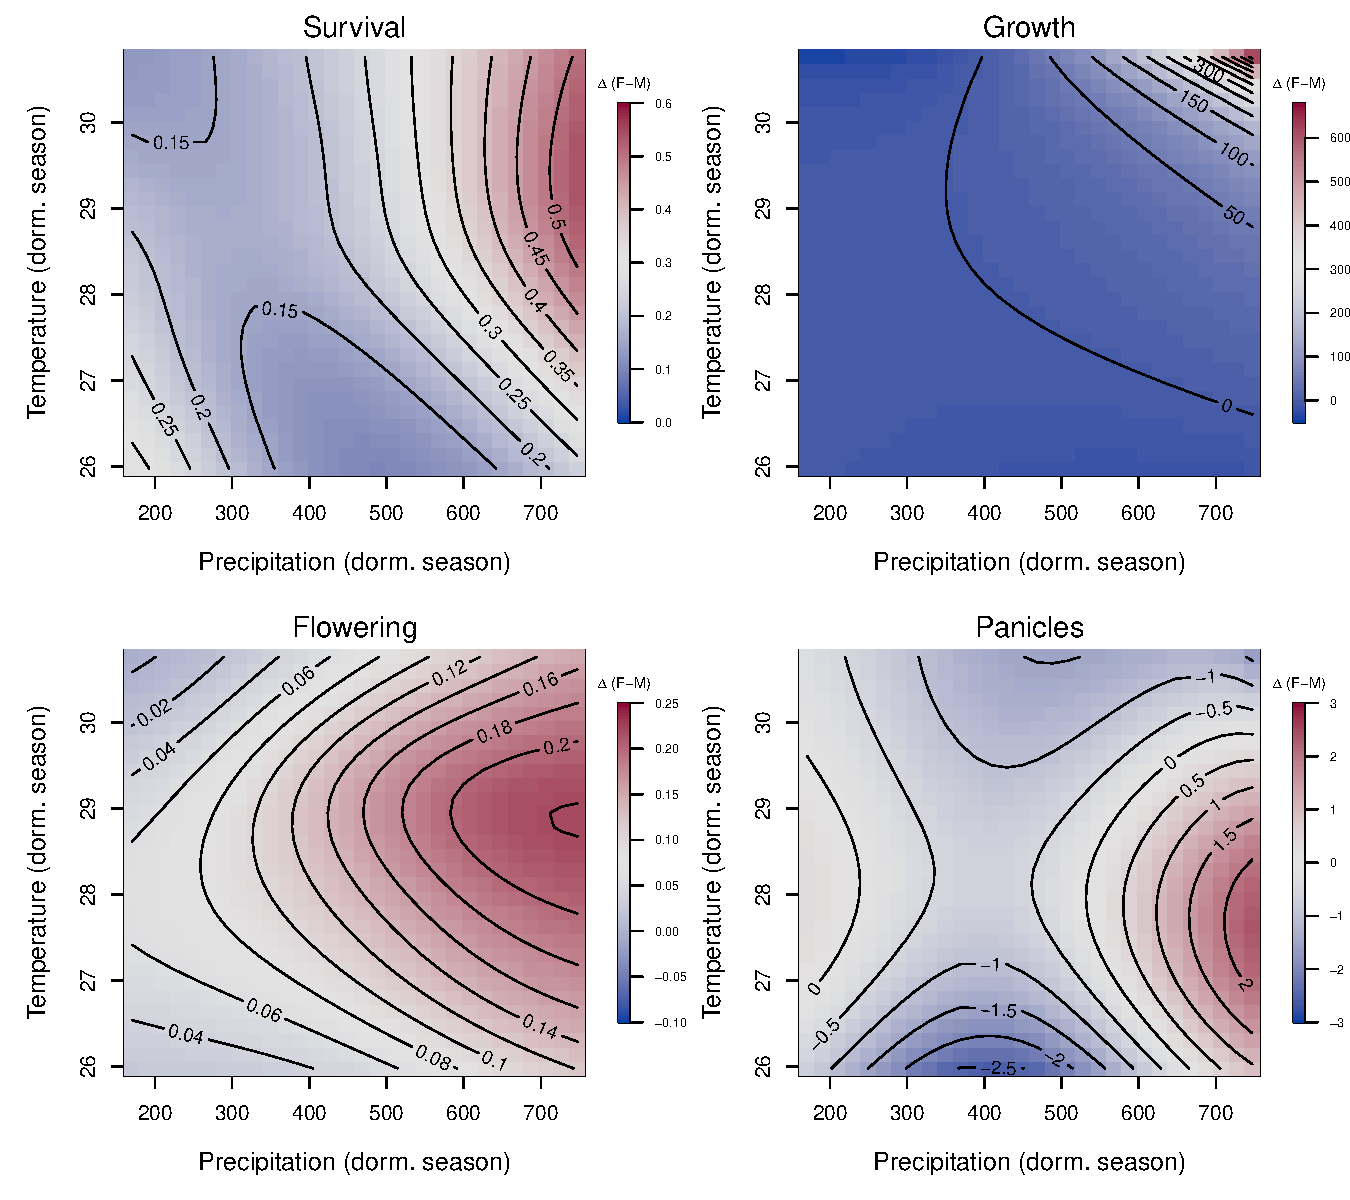
\includegraphics[width=0.99\linewidth]{Figures/Vital_rate_dormant_3D.pdf}
	\caption{ Predicted difference in demographic response to climate across species range between female and male. Contours show predicted value of that difference conditional on precipitation and temperature of the dormant  season }
	\label{Sup:vt_3D_dorm}
\end{figure}

\begin{figure}[H]
	\begin{center}
		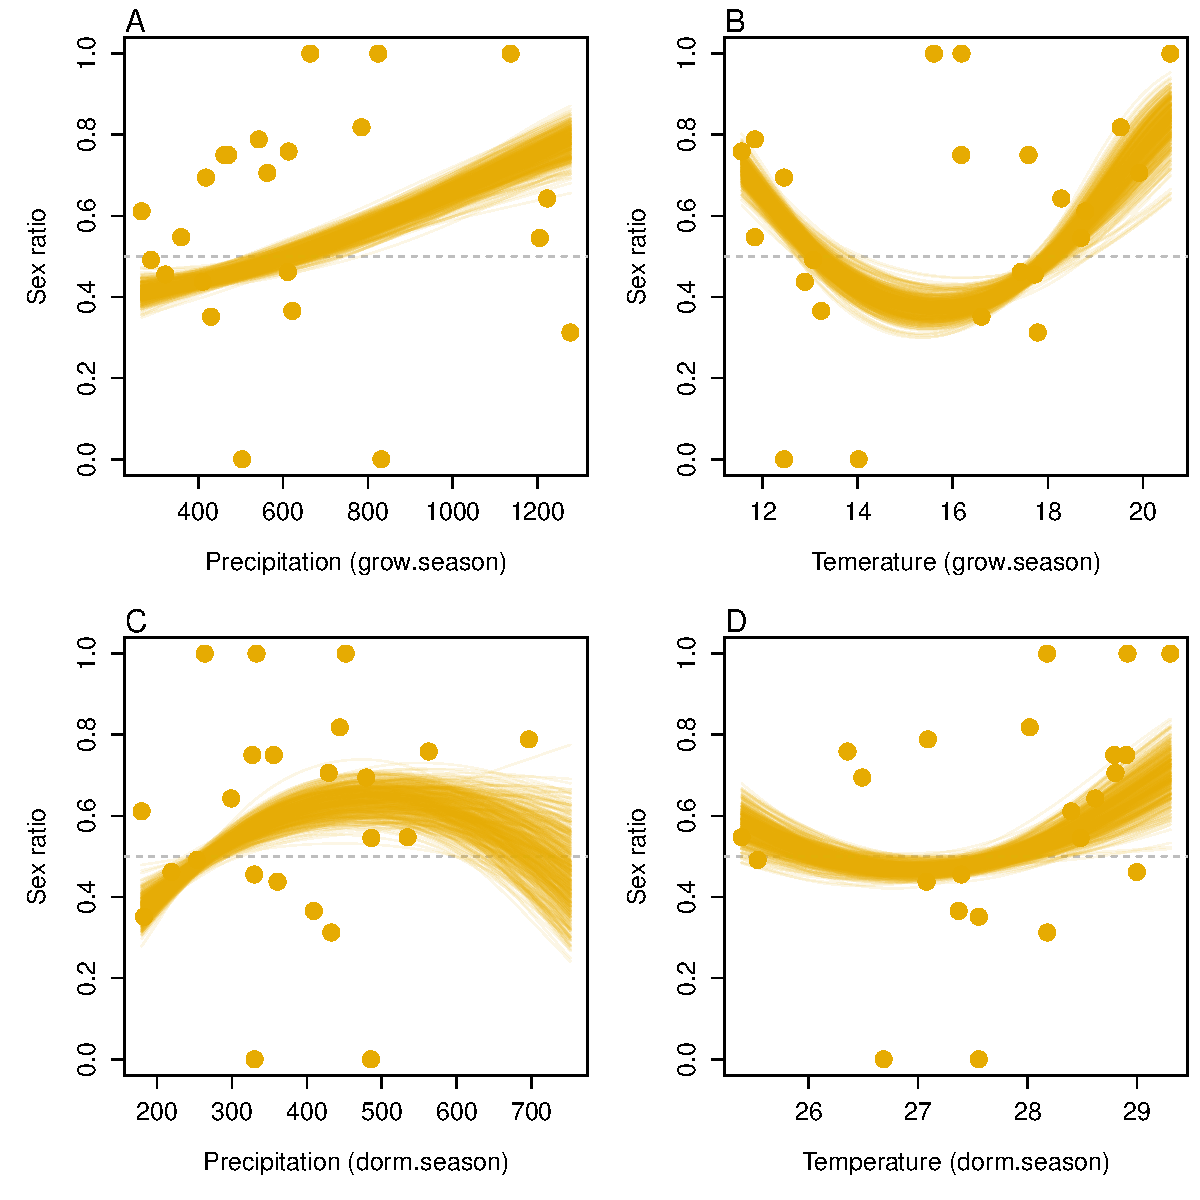
\includegraphics[width=0.95\linewidth]{Figures/gardens_OSR.pdf}
		\caption{\textbf{Significant Operational Sex Ratio response across climate gradient}.
			(A, B) Proportion of panicles that were females across  temperature of the growing and dormant season }
		\label{Sup:gardens_OSR}
	\end{center}
\end{figure}

\begin{figure}[H]
	\begin{center}
		\includegraphics[width=0.70\linewidth]{Figures/Posterior_ORS.pdf}
		\caption{Mean parameter values and 95\% credible intervals of the posterior probability distributions. 
		pptgrow is  the precipitation of growing season,
		Tempgrow is the temperature of growing season,
		pptdorm is the temperature of dormant season,
		Tempdorm is the temperature of dormant season.}
		\label{Sup:posterior_OSR}
	\end{center}
\end{figure}


%\begin{figure}[H]
%	\begin{center}
%		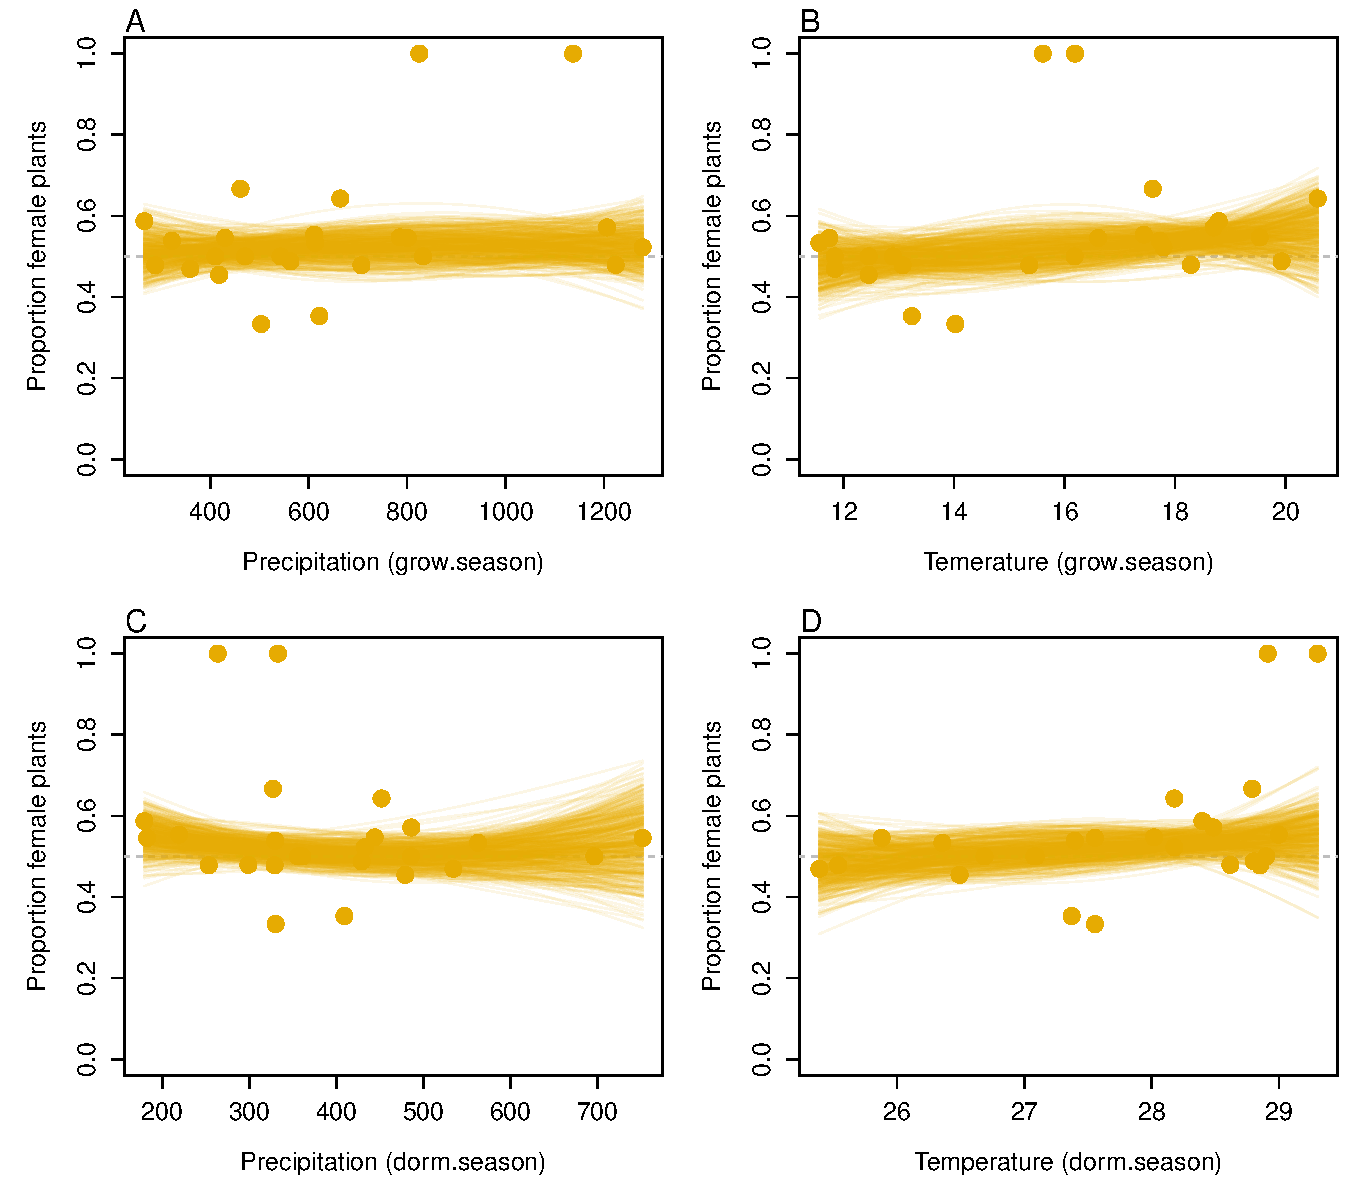
\includegraphics[width=0.80\linewidth]{Figures/gardens_SR.pdf}
%		\caption{\textbf{Variation in sex-ratio accross climate gradient}.
%			(A, B) Proportion of plants that were females across precipitation and temperature of the growing season; (C, D) Proportion of plants that were females across precipitation and temperature of the dormant season.}
%		\label{Sup:gardens_SR}
%	\end{center}
%\end{figure}

%\begin{figure}[H]
%	\centering
%	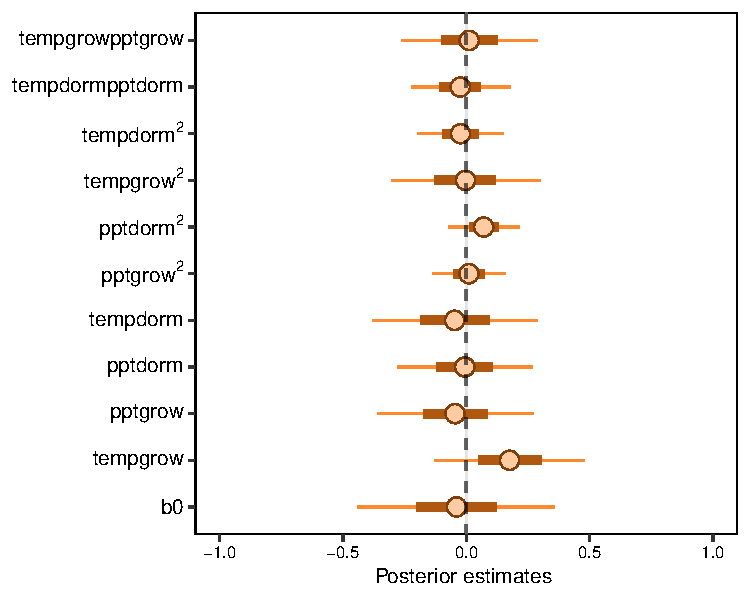
\includegraphics[width=0.5\linewidth]{Figures/Posterior_SR.pdf}
%	\caption{Mean parameter values and 95\% credible intervals of the posterior probability distributions. 
%		pptgrow is  the precipitation of growing season,
%		Tempgrow is the temperature of growing season,
%		pptdorm is the temperature of dormant season,
%		Tempdorm is the temperature of dormant season.}
%	\label{Sup:PosteriorSR}
%\end{figure}

% \begin{figure}[H]
%   \begin{center}
%     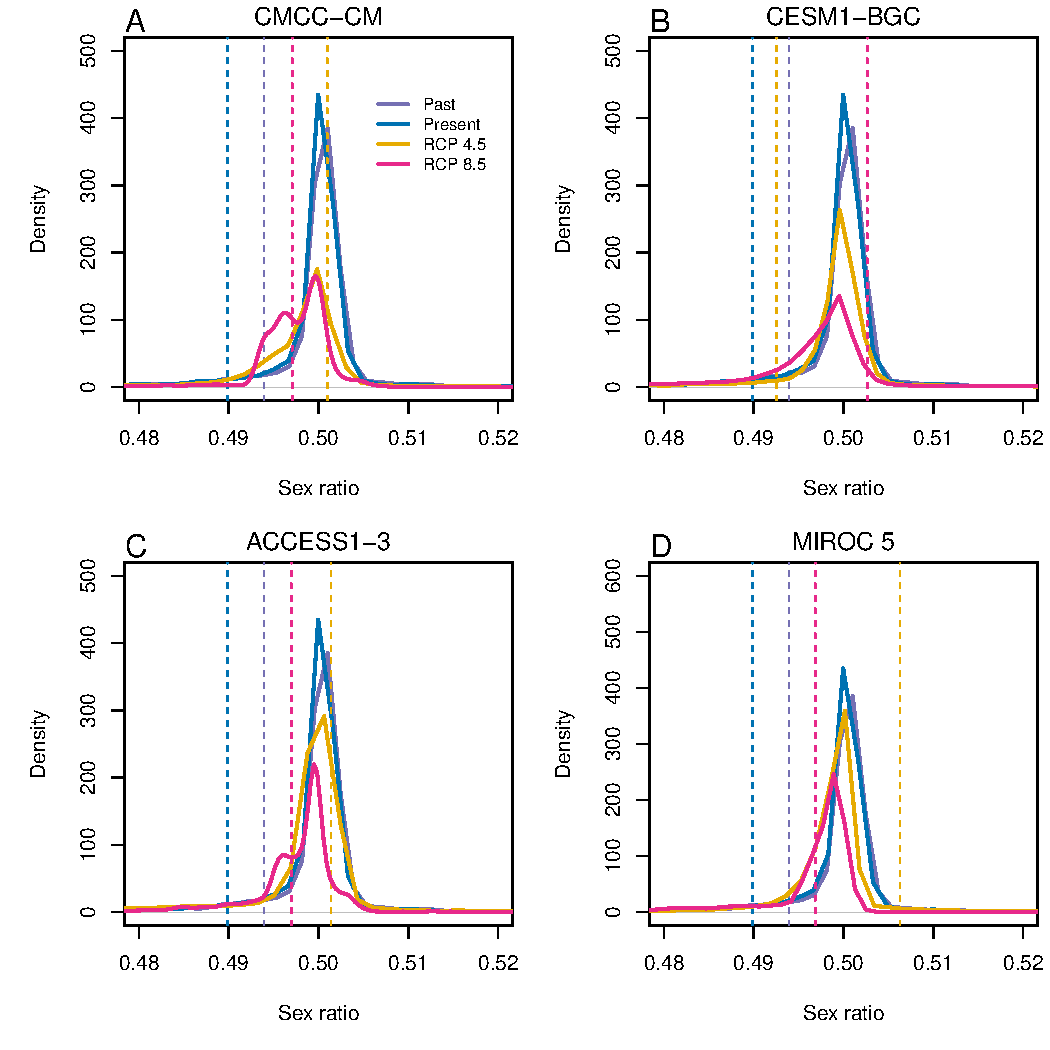
\includegraphics[width=0.99\linewidth]{Figures/POAR_SR.pdf}
%   \caption{Change in Sex ratio (proportion of female) over time (past, present, future).
%   The means for each model are shown as vertical dashed lines.}
%   \label{Sup:srall}
%   \end{center}
% \end{figure}

\begin{figure}[H]
	\begin{center}
		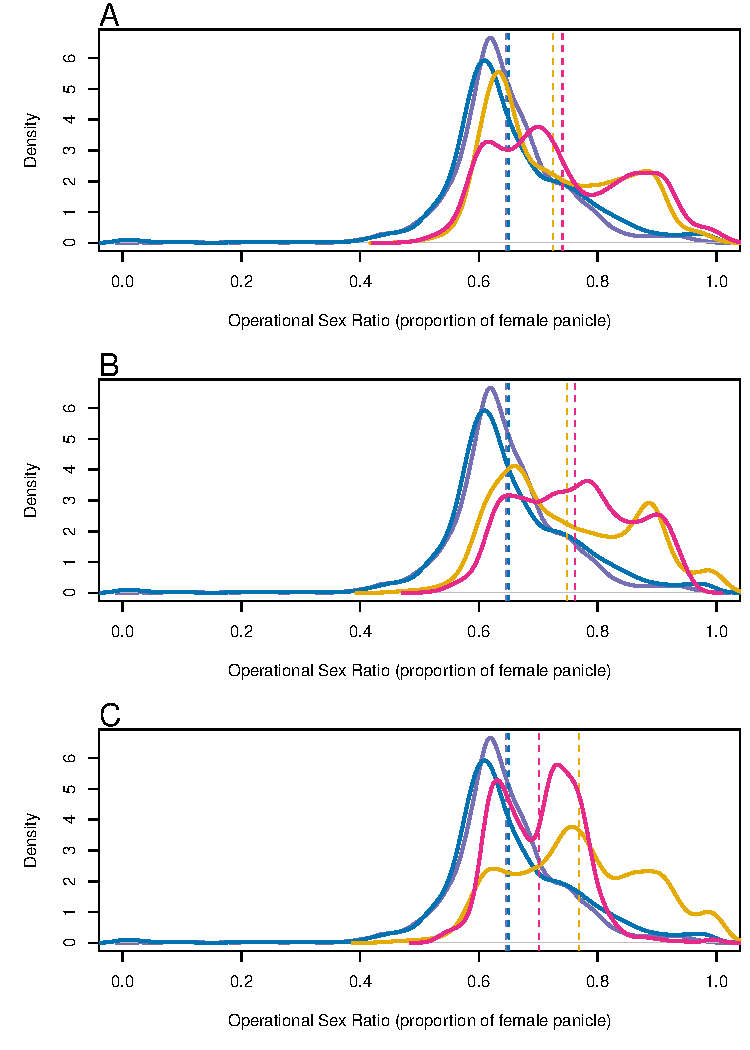
\includegraphics[width=0.80\linewidth]{Figures/POAR_OSR_MIROC_CES_ACC.pdf}
		\caption{Change in Operational Sex Ratio (proportion of female) over time (past, present, future).
			Future projections were based on A) MIROC 5, B) CES, C) ACC.
			The means for each model are shown as vertical dashed lines.}
		\label{Sup:osrall}
	\end{center}
\end{figure}

\begin{figure}[H]
	\begin{center}
		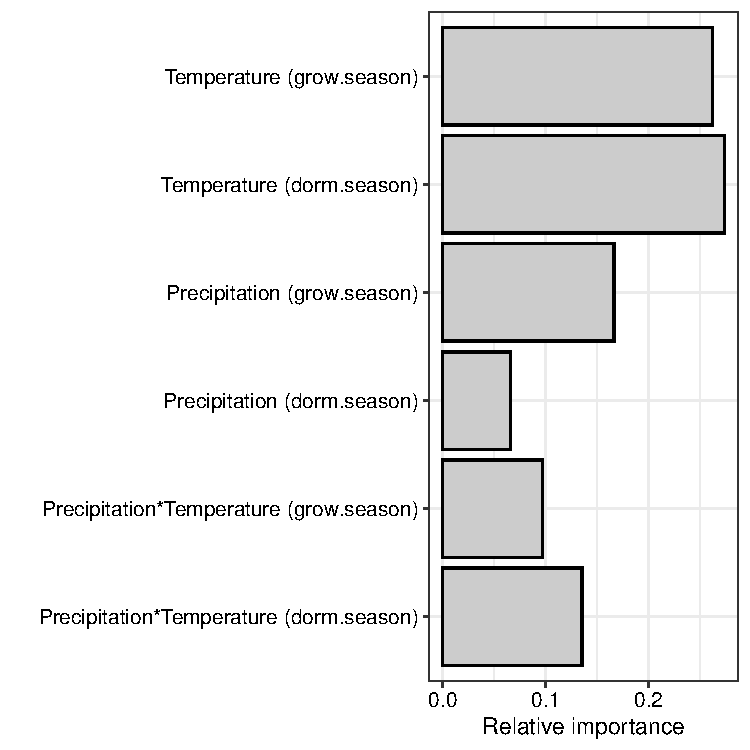
\includegraphics[width=0.65\linewidth]{Figures/Fig_LTRE.pdf}
		\caption{Life Table Response Experiment: The bar represent the relative importance of each predictors.}
		\label{Sup:LTRE}
	\end{center}
\end{figure}

\begin{figure}[H]
	\begin{center}
		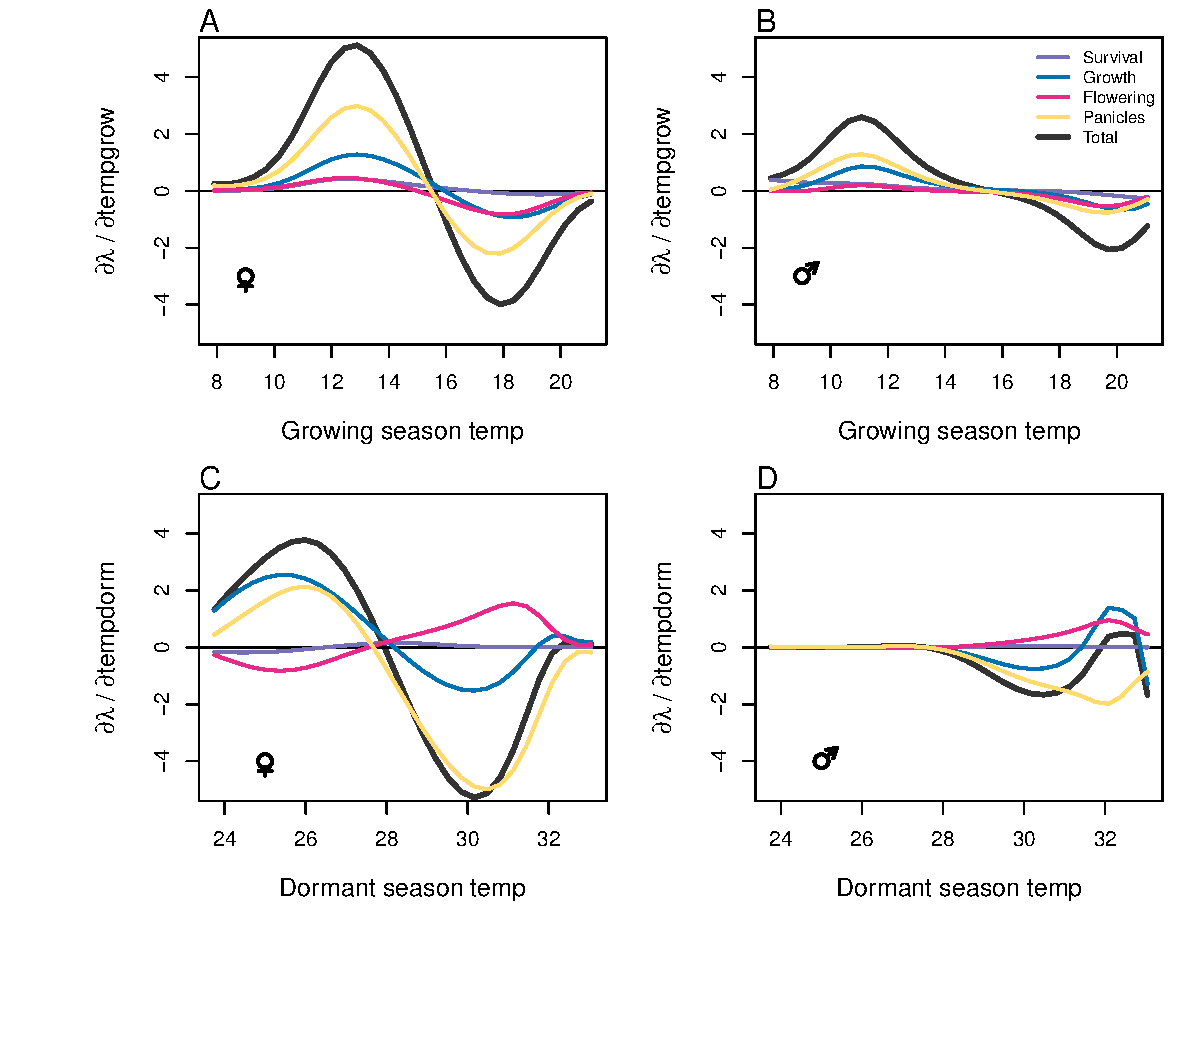
\includegraphics[width=0.95\linewidth]{Figures/LTRE_Temperature.pdf}
		\caption{Life table response experiment decomposition of the sensitivity of $\lambda$ to seasonal climate into additive vital rate contributions of males and females based on posterior mean parameter estimates.
			(A) Temperature of growing season (contribution of female), (B) Temperature of growing season (contribution of male),  (C) Temperature of dormant season (contribution of female) and (D) Temperature of dormant season (contribution of male).}
		\label{Sup:LTRETemp}
	\end{center}
\end{figure}

%\begin{figure}[H]
%	\begin{center}
%		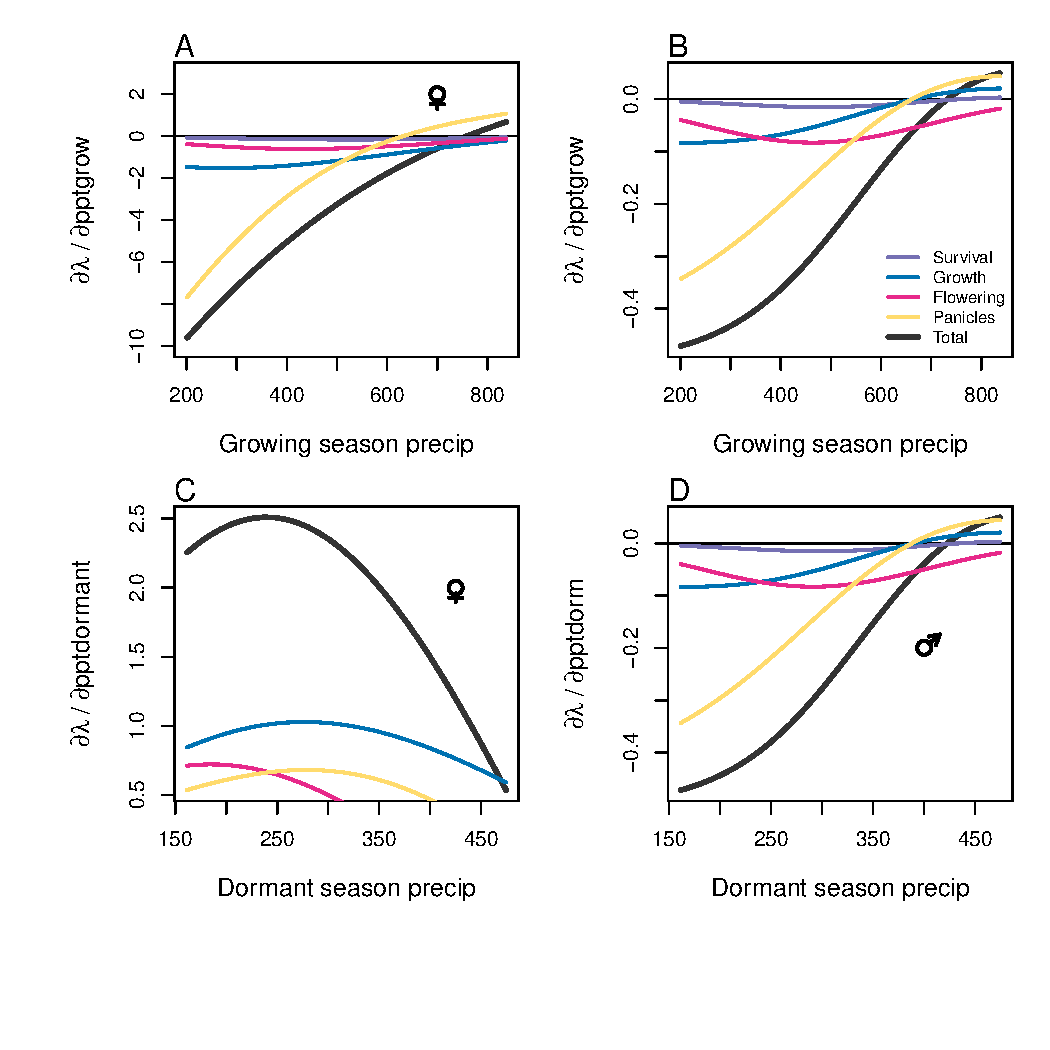
\includegraphics[width=0.95\linewidth]{Figures/LTRE_Precipitation.pdf}
%		\caption{Life table response experiment decomposition of the sensitivity of $\lambda$ to seasonal climate into additive vital rate contributions of males and females based on posterior mean parameter estimates.
%			(A) Precipitation of growing season (contribution of female), (B) Precipitation of growing season (contribution of male),  (C) Precipitation of dormant season (contribution of female) and (D) Precipitation of dormant season (contribution of male).}
%		\label{Sup:LTREppt}
%	\end{center}
%\end{figure}

\begin{figure}[H]
	\begin{center}
		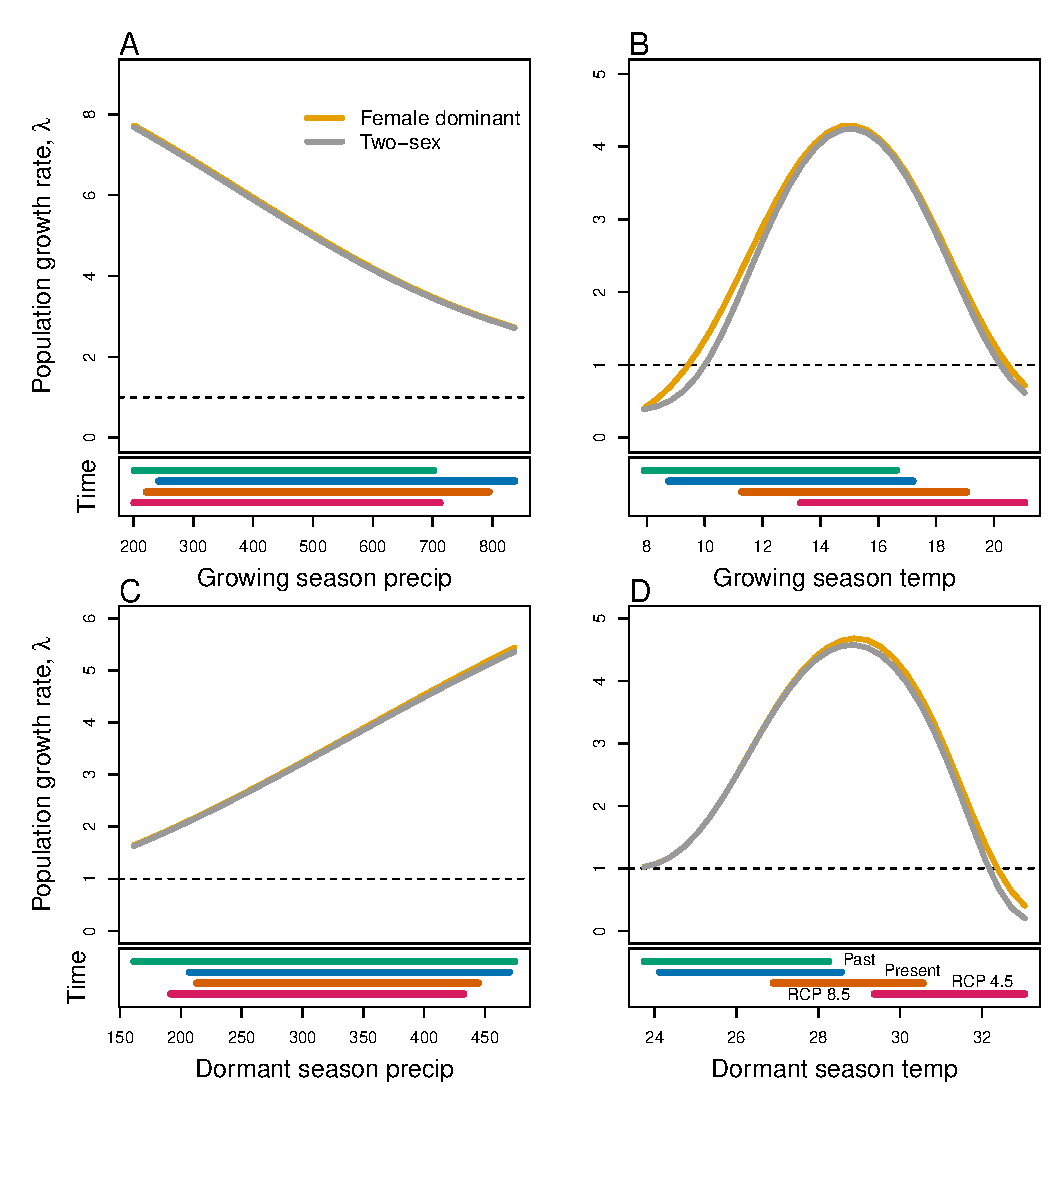
\includegraphics[width=1\linewidth]{Figures/lambda_past_present_future.pdf}
		\caption{\textbf{Predicted population growth rate ($\lambda$) in different ranges of climate}.
			(A) Precipitation of the growing season, (B) Temperature of the growing season, (C) Precipitation of the dormant season, (D) Temperature of the dormant season.
			The grey curve shows prediction by the two-sex matrix projection model that incorporates sex- specific demographic responses to climate with sex ratio dependent seed fertilization.
			The orange curve represents the prediction by the female dominant matrix projection model.
			The dashed horizontal line indicates the limit of population viability ($\lambda$ = 1).
			Lower panels below each data panel shows  ranges of climate values for different time period (past climate, present and future climates).
			For future climate, we show a Representation Concentration Pathways (RCP) 4.5 and 8.5. Values of ($\lambda$) are derived from the mean climate variables across 4 GCMs (MIROC5, ACCESS1-3, CESM1-BGC, CMCC-CM).
			% Life table response experiment decomposition of the sensitivity of $\lambda$ to seasonal climate into additive vital rate contributions of males and females based on posterior mean parameter estimates.
			%  (A) Temperature of growing season (contribution of female), (B) Temperature of growing season (contribution of male),  (C) Temperature of dormant season (contribution of female) and (D) Temperature of dormant season (contribution of male).
		}
		\label{fig:lambda_LTRE}
	\end{center}
\end{figure}


\begin{figure}[H]
	\begin{center}
		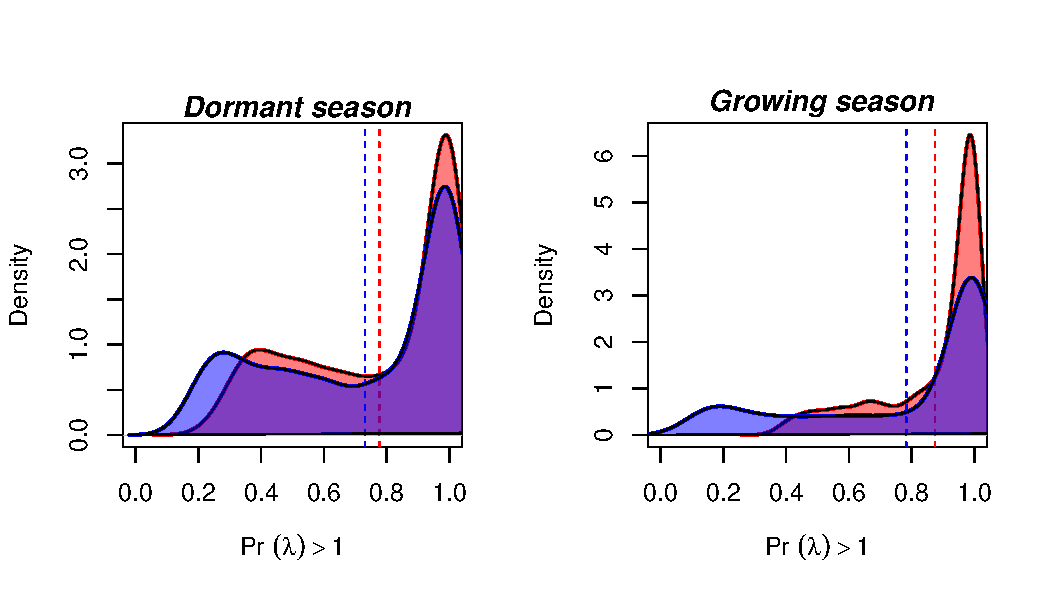
\includegraphics[width=0.99\linewidth]{Figures/Niche_overestimation.pdf}
		\caption{ Assessment of the statistical difference between the two-sex models and the female dominant model for the dormant and growing season. 
			Plots show the density of Pr ($\lambda$) > 1 values for female dominant (pink) and two-sex models (violet) for each season. 
			The means for each model are shown as vertical dashed lines. }
		\label{Sup:Niche_overestimation}
	\end{center}
\end{figure}

% \begin{figure}[H]
%   \begin{center}
%     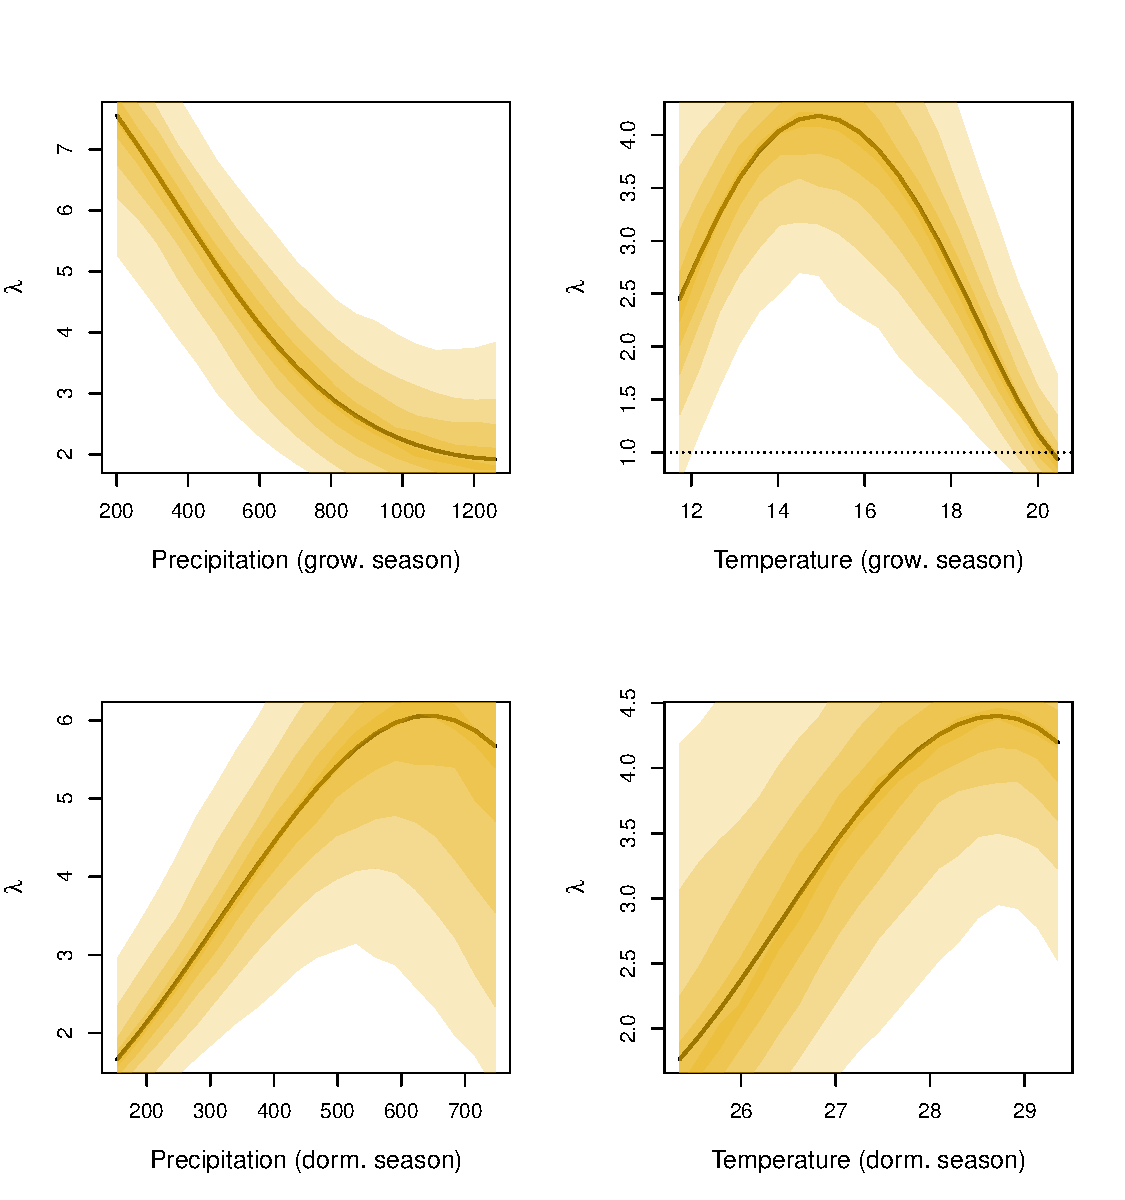
\includegraphics[width=0.95\linewidth]{Figures/lambda_CI.pdf}
%   \caption{Population growth rate ($\lambda$) as a function of seasonal climate (2015-2017), predicted by the two-sex matrix projection model that incorporates sex-specific demographic responses to climate with sex ratio-dependent seed fertilization.
% We show the mean posterior distribution of $\lambda$ in solid lines, and the 5, 25, 50, 75, and 95\% percentiles of parameter uncertainty in shaded gold color.
% The dashed horizontal line indicates the limit of population viability ($\lambda$ = 1)}
%   \label{Sup:lambda2sex}
%   \end{center}
% \end{figure}

\begin{figure}[H]
	\begin{center}
		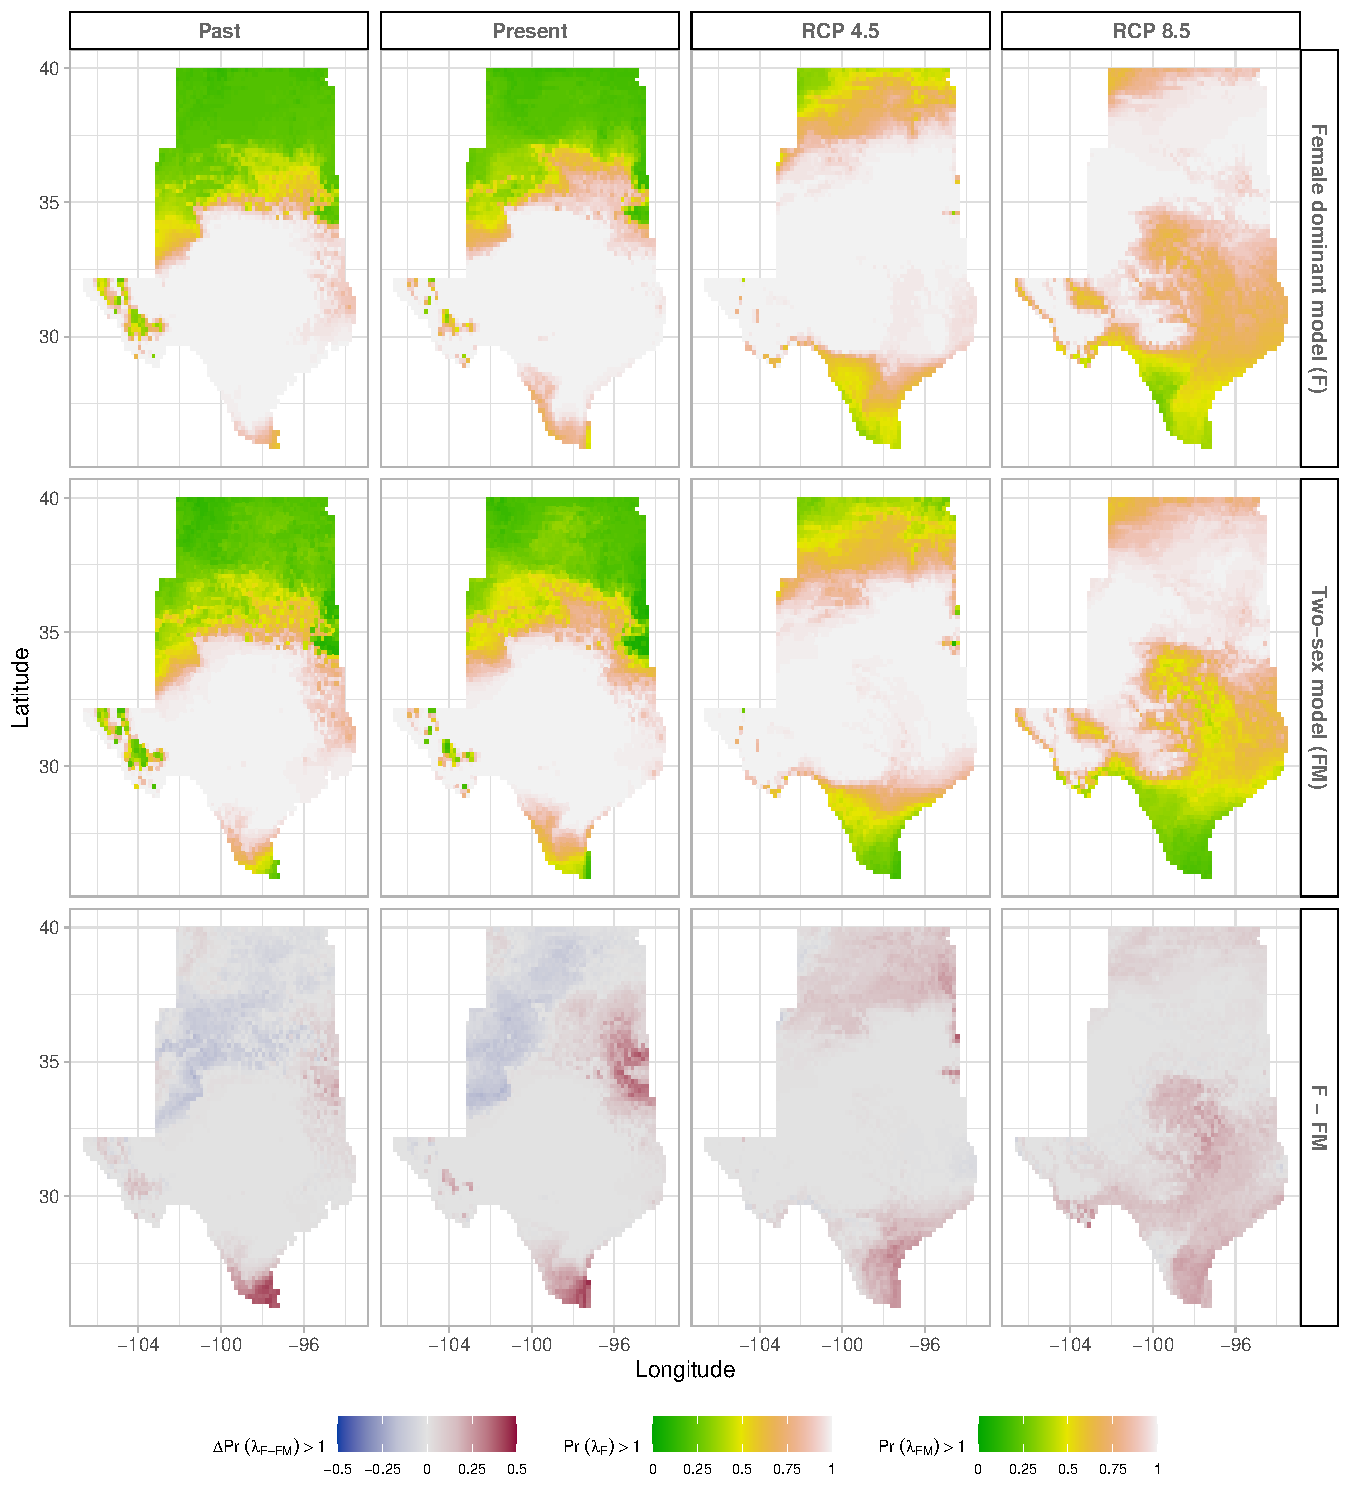
\includegraphics[width=0.95\linewidth]{Figures/Fig_geoPrlambda_ces.pdf}
		\caption{Climate change favors range shift toward the North edge of the current range.
			(A) Past, (B) Current, (C and D) Future predicted range shift based on the predicted probabilities of self- sustaining populations, Pr ($\lambda > 1$), using the two-sex model that incorporates sex- specific demographic responses to climate with sex ratio dependent seed fertilization.
			(E) Past, (F) Current, (G and F) Future  predicted range shift based on the predicted probabilities of self- sustaining populations, Pr ($\lambda > 1$), using the female dominant model.
			Future projections were based on the CESM1-BGC model.
			The black dots on panel B and F indicate all known presence points collected from GBIF from 1990 to 2019, which corresponds to the current condition in our prediction. 
			The occurrences of GBIFs are distributed in with higher population fitness habitat Pr ($\lambda$ > 1) , confirming that our study approach can reasonably predict range shifts. }
		\label{Sup:geoprojces}
	\end{center}
\end{figure}

\begin{figure}[H]
	\begin{center}
		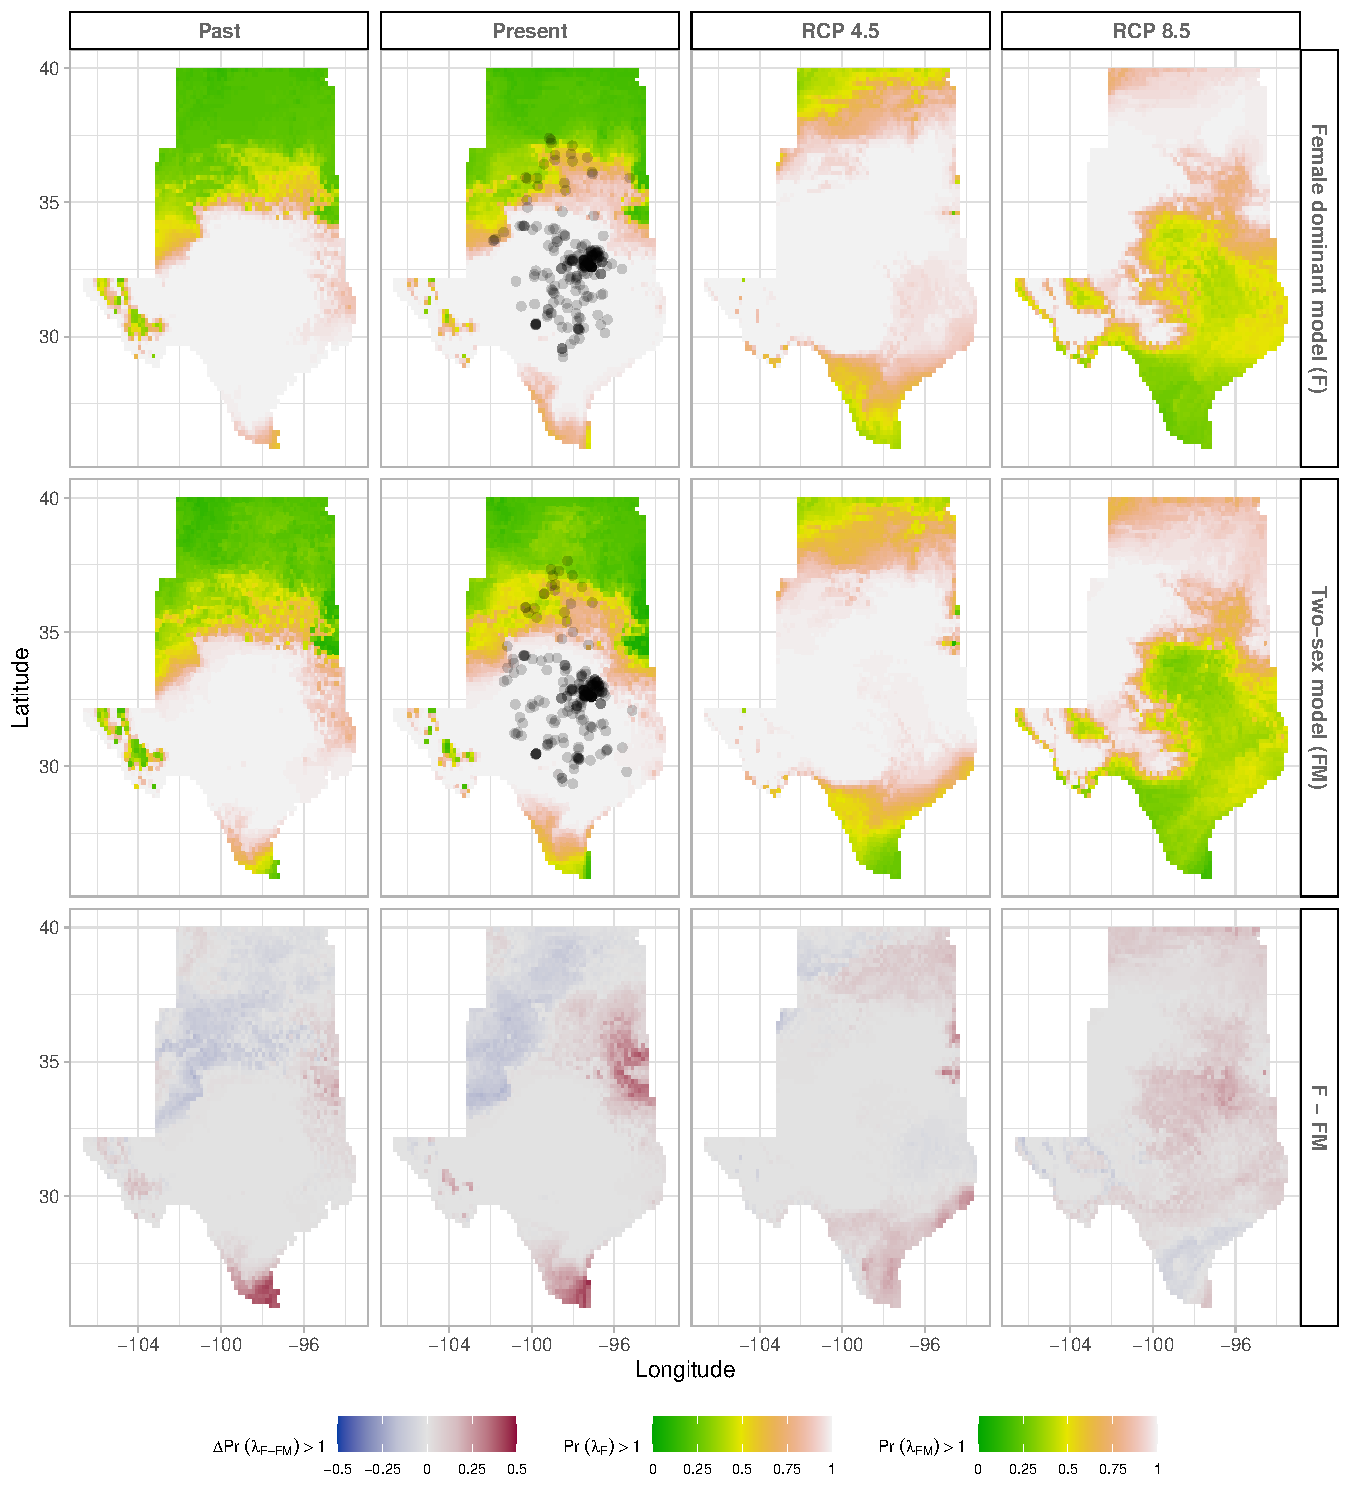
\includegraphics[width=0.95\linewidth]{Figures/Fig_geoPrlambdaacc.pdf}
		\caption{Climate change favors range shift toward the North edge of the current range.
			(A) Past, (B) Current, (C and D) Future predicted range shift based on the predicted probabilities of self- sustaining populations, Pr ($\lambda > 1$), using the two-sex model that incorporates sex- specific demographic responses to climate with sex ratio dependent seed fertilization.
			(E) Past, (F) Current, (G and F) Future  predicted range shift based on the predicted probabilities of self- sustaining populations, Pr ($\lambda > 1$), using the female dominant model.
			Future projections were based on the  ACCESS model.
			The black dots on panel B and F indicate all known presence points collected from GBIF from 1990 to 2019, which corresponds to the current condition in our prediction. 
			The occurrences of GBIFs are distributed in with higher population fitness habitat Pr ($\lambda$ > 1) , confirming that our study approach can reasonably predict range shifts.}
		\label{Sup:geoprojacc}
	\end{center}
\end{figure}

\begin{figure}[H]
	\begin{center}
		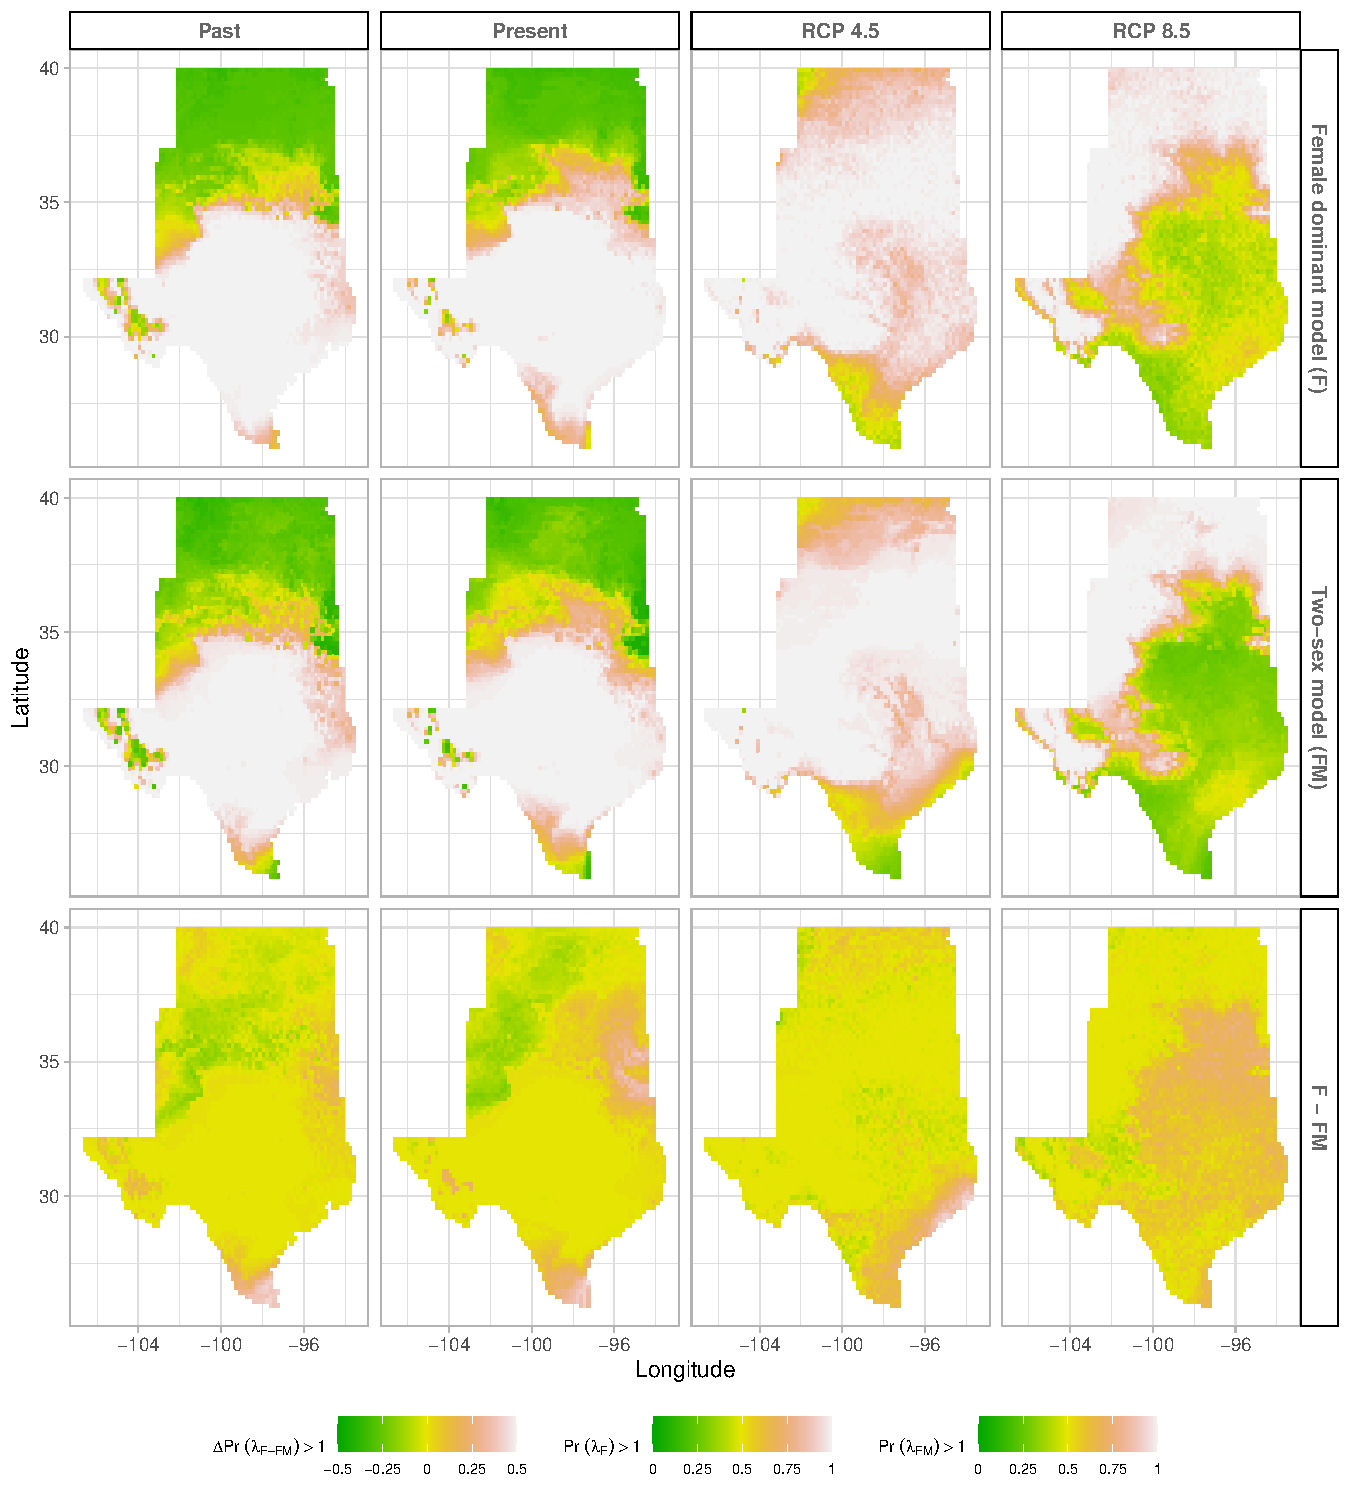
\includegraphics[width=0.95\linewidth]{Figures/Fig_geoPrlambda_miroc.pdf}
		\caption{Climate change favors range shift toward the North edge of the current range.
			(A) Past, (B) Current, (C and D) Future predicted range shift based on the predicted probabilities of self- sustaining populations, Pr ($\lambda > 1$), using the two-sex model that incorporates sex- specific demographic responses to climate with sex ratio dependent seed fertilization.
			(E) Past, (F) Current, (G and F) Future  predicted range shift based on the predicted probabilities of self- sustaining populations, Pr ($\lambda > 1$), using the female dominant model.
			Future projections were based on the MIROC5 model.
			The black dots on panel B and F indicate all known presence points collected from GBIF from 1990 to 2019, which corresponds to the current condition in our prediction. 
			The occurrences of GBIFs are distributed in with higher population fitness habitat Pr ($\lambda$ > 1) , confirming that our study approach can reasonably predict range shifts.}
		\label{Sup:geoprojmiroc}
	\end{center}
\end{figure}

\begin{figure}[H]
	\begin{center}
		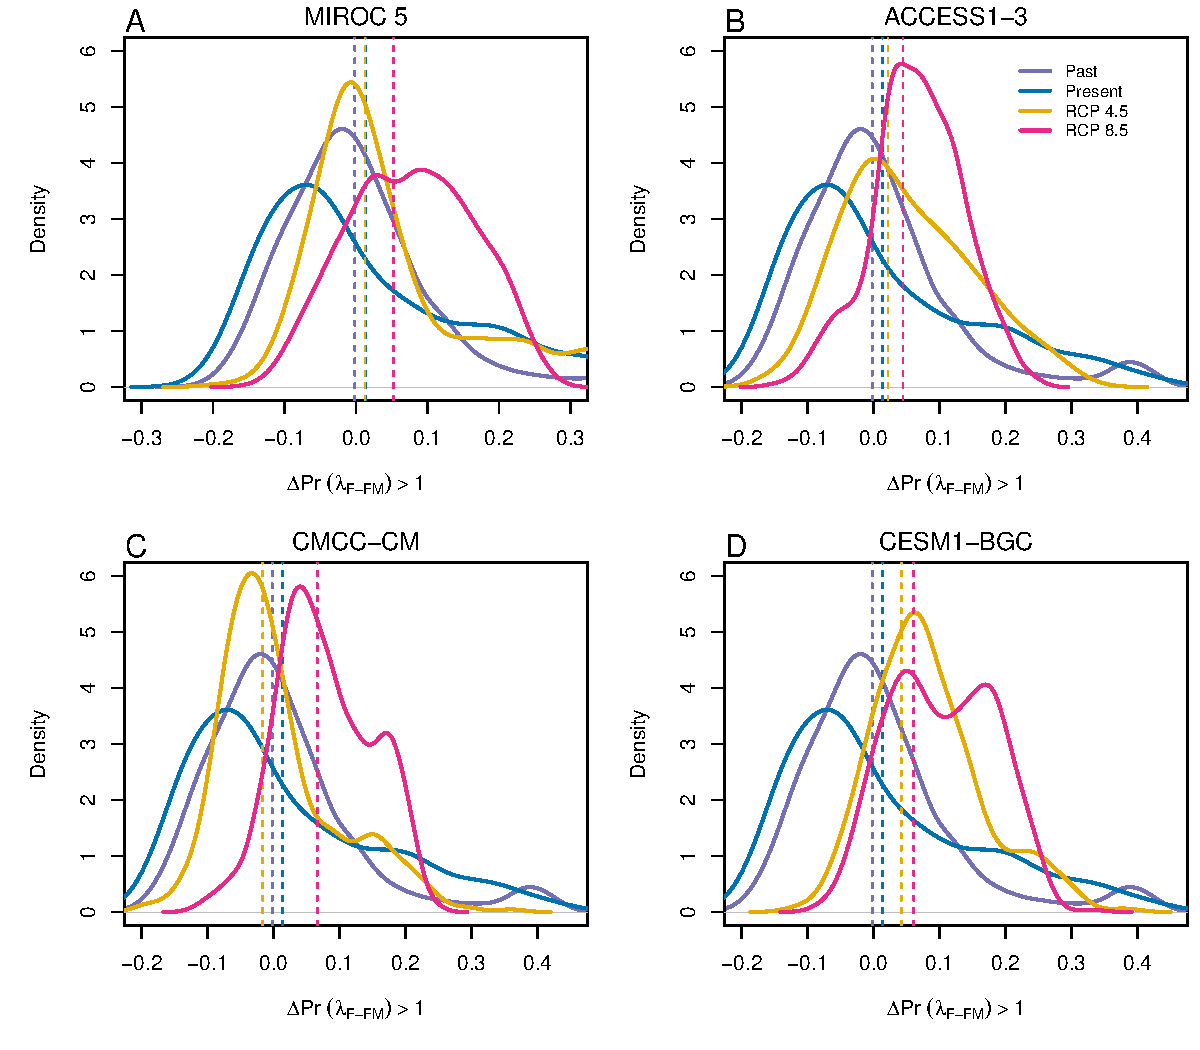
\includegraphics[width=0.99\linewidth]{Figures/Densityplot_lambda_GCMs.pdf}
		\caption{ Assessment of the statistical difference between the two-sex models and the female dominant model across and beyond species range for 4 GCMs. 
			The means for each model are shown as vertical dashed lines. }
		\label{Sup:geo_overestimation}
	\end{center}
\end{figure}

% \begin{figure}[H]
%   \begin{center}
%     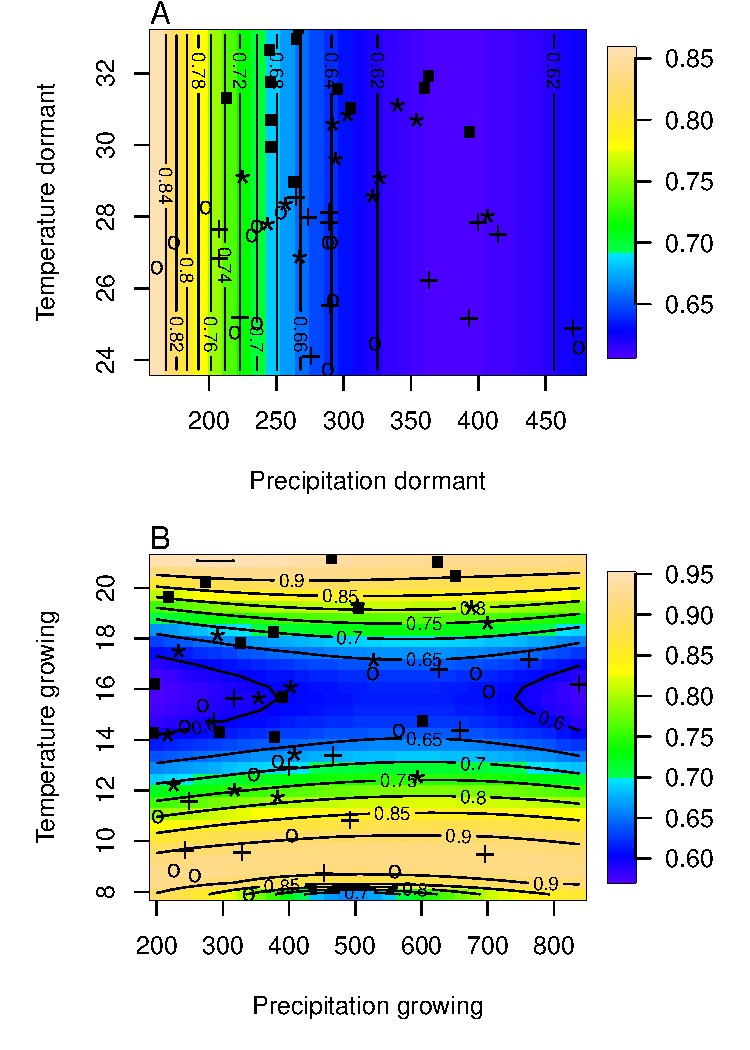
\includegraphics[width=0.75\linewidth]{Figures/OSR.pdf}
%   \caption{A two‐dimensional representation of the Operational Sex Ratio (OSR) over time (past, present and future climate conditions). 
%   OSR represents the proportion of females. 
%   Contours show predicted values of OSR conditional on precipitation and temperature of the dormant and growing season.
%   Operational Sex Ratio during the dormant season for the two sex model (A), Operational Sex Ratio during the growing season for the two sex model (B).
%   "\begin{normalsize}\textbf{o}\end{normalsize}": Past, "\begin{normalsize}\textbf{+}\end{normalsize}": Current,"\begin{large}\textbf{*}\end{large}": RCP 4.5,"\begin{tiny}$\blacksquare$\end{tiny}": RCP 8.5.}
%   \label{Sup:OSR}
%   \end{center}
% \end{figure}

% \begin{figure}[H]
%   \begin{center}
%     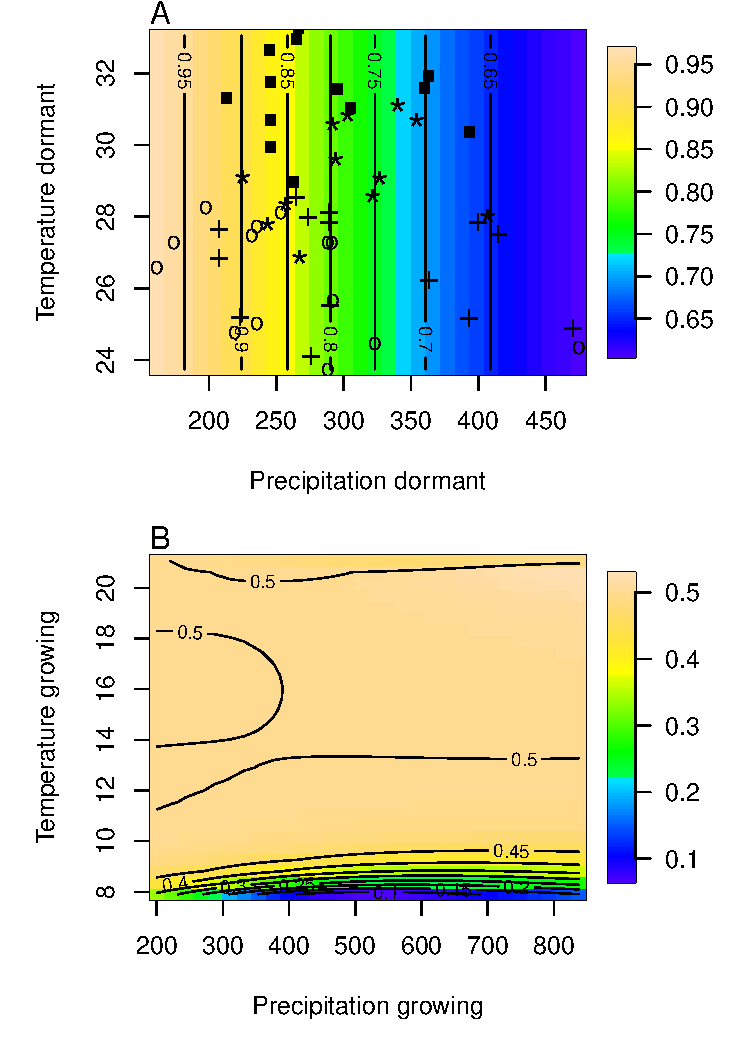
\includegraphics[width=0.85\linewidth]{Figures/SR.pdf}
%   \caption{A two‐dimensional representation of the  Sex Ratio (SR) over time (past, present and future climate conditions). 
%   Contours show predicted values of SR conditional on precipitation and temperature of the dormant and growing season.
%   Sex Ratio during the dormant season for the two sex model (A),Sex Ratio during the growing season for the two sex model (B).}
%   \label{Sup:SR}
%   \end{center}
% \end{figure}

\section {Supporting Methods}

\subsection{Sex-specific demographic responses to climatic variation across common garden sites} \label {sssec:vital_rate}
Vital rate models were fit with the same linear predictors for the expected value ($\mu$)(Eq.\ref{eq:mu}):
\begin{align}\label{eq:mu}
\begin{split}
\mu = \beta_{0} + \beta_{1}size + \beta_{2}sex + \beta_{3}pptgrow + \beta_{4}pptdorm + \beta_{5}tempgrow + \beta_{6}tempdorm \\ 
+ \beta_{7}pptgrow*sex + \beta_{8}pptdorm*sex + \beta_{9}tempgrow*sex + \beta_{10}tempdorm*sex  \\ 
+  \beta_{11}size*sex + \beta_{12}pptgrow*tempgrow + \beta_{13}pptdorm*tempdorm\\
+ \beta_{14}pptgrow*tempgrow*sex + \beta_{15}pptdorm*tempdorm*sex + \beta_{16}pptgrow^2\\
+ \beta_{17}pptdorm^2 + \beta_{18}tempgrow^2 + \beta_{19}tempdorm^2 + \beta_{20}pptgrow^2*sex  \\
+ \beta_{21}pptdorm^2*sex + \beta_{22}tempgrow^2*sex + \beta_{23}tempdorm^2*sex + \phi + \rho + \nu 
\end{split}
\end{align}
\noindent where $\beta_{0}$ is the  grand mean intercept, $\beta_{1}$ is the size dependent slopes.
$size$ was on a natural logarithm scale. 
$\beta_{2}$...$\beta_{13}$ represent the climate dependent slopes.
$\beta_{14}$...$\beta_{23}$ represent the sex-climate interaction slopes.
$pptgrow$ is the precipitation of the growing season, $tempgrow$ is the temperature of the growing season, $pptdorm$ is the precipitation of the dormant season, $tempdorm$ is the temperature of the dormant season.

\subsection{Sex ratio responses to climatic variation across common garden sites} \label {sssec:sexratio_bayesian}
To understand the impact of climatic variation across common garden sites on sex ratio, OSR and SR  models using  the same linear predictors for the expected value ($\nu$)(Eq.\ref{eq:sr_fn}):
\begin{align}\label{eq:sr_fn}
\begin{split}
	\nu =   \omega_{0}+ \omega_{1}pptgrow + \omega_{2}pptdorm + \omega_{3}tempgrow + \omega_{4}tempdorm + \\
	  \omega_{5}pptgrow^2 + \omega_{6}pptdorm^2 + \omega_{7}tempgrow^2 + \omega_{8}tempdorm^2 + \epsilon\\
\end{split}
\end{align}
\noindent where $OSR$ is the proportion of panicles that were female or proportion of female individuals in the experimental populations, c is the climate. 
$\omega_{0}$ is the intercept, $\omega_{1}$, .... $\omega_{8}$ are the climate dependent slopes. $\epsilon$ is error term.

\subsection{Sex ratio experiment} \label {sssec:experiment}
To estimate the probability of seed viability,  the germination rate and the effect of sex-ratio variation on female reproductive success, we conducted a sex-ratio experiment at one site near the center of the range to estimate the effect of sex-ratio variation on female reproductive success.
The details of the experiment are provided in \cite{compagnoni2017can} and \cite{miller2022two}.
Here we provide a summary of the experiment.
We established 124 experimental populations in plots measuring 0.4 x 0.4m and separated by at least 15m from each other.
We varied population density (1-48 plants/plot) and sex ratio (0\%-100\% female) across the experimental populations, and we replicated 34 combinations of density and sex ratio.
We collected panicles from a subset of females in each plot and recorded the number of seeds in each panicle.
We assessed reproductive success (seeds fertilized) using greenhouse-based germination and trazolium-based seed viability assays.
Seed viability was modeled with a binomial distribution where the probability of viability ($v$) was given by:
\begin{align}\label{eq:viab}
	v = v_{0} * (1 - OSR^{\alpha})
\end{align}
\noindent where $OSR$ is the proportion of panicles that were female in the experimental populations.
% The properties of the above function is supported by our previous work \citep{compagnoni2017can}.
% Here, seed viability is maximized at $v_{0}$ as $OSR$ approaches zero (strongly male-biased) and goes to zero as $OSR$ approaches $1$ (strongly female-biased).
$\alpha$ is the parameter that control for how viability declines with increasing female bias.
Further, germination rate was modeled using a binomial distribution to model the germination data from greenhouse trials.
Given that germination was conditional on seed viability, the probability of success was given by the product $v*g$, where $v$ is a function of $OSR$ (Eq. \ref{eq:viab}) and $g$ is assumed to be constant.

\end{document}
